\section{Introduction}
\label{sec:intro}

Sparse Merkle Trees (SMTs) are Merkle trees over large logical address spaces. A height-$h$ SMT has $2^h$ possible leaf coordinates, but only a small subset of leaves is usually occupied. Empty subtrees are represented by publicly known default hashes. This default-hash mechanism makes SMTs a common building block for revocation maps, authenticated dictionaries, and blockchain state commitments~\cite{sparsemt,revtrans,jmt,ethereum,zcash}. Despite the sparse representation, membership verification keeps the standard Merkle proof interface: a verifier checks a leaf value together with one sibling digest per level and recomputes the committed root.

The standard SMT proof API is efficient, but it reveals the queried target. When a client requests a membership proof, the server learns which key, account, certificate, or state object is being checked, and it also observes the corresponding authenticated path. Existing SMT work mainly improves storage, proof generation, multiproofs, and updates. These optimizations reduce the cost of proof serving, but they do not provide query privacy. This paper studies private retrieval of SMT membership proofs for a fixed public snapshot: the snapshot and its public metadata may be known, while the queried occupied leaf should remain hidden.

Private information retrieval (PIR) is the natural tool for hiding a database index, but an SMT membership proof is not a single database record. A standard proof is a height-$h$ array of sibling digests. Some of these digests are non-default values that must be obtained from the server, while others are default hashes that the client can reconstruct locally from the public default-hash chain. Running one independent PIR query per proof level would hide the target, but it would treat a structured Merkle proof as $h$ unrelated private lookups.

Thus, private SMT proof retrieval is better viewed as a structured batch-PIR problem. The client must retrieve several sibling digests using a target-independent query pattern, without revealing which Merkle path those digests belong to. Generic batch-PIR techniques can privately retrieve multiple records, but they treat the requested records as an arbitrary set. This line includes classical batch codes and combinatorial batch codes~\cite{batchcodes,cbc}, probabilistic batch codes (PBCs) as used in SealPIR~\cite{sealpir}, and recent multi-query PIR systems such as Vectorized BatchPIR and PIRANA~\cite{vectorbatchpir,pirana}. These systems improve the cryptographic or coding layer, but they do not decide which SMT proof elements should be stored in the PIR database, and they do not specify how the client should reconstruct the complete height-$h$ proof using public default hashes.

Merkle proofs provide additional structure: all required sibling digests are determined by one root-to-leaf path. TreePIR~\cite{treepir} exploits this structure for perfect binary Merkle trees by coloring proof nodes so that each proof path contains at most one node of each color, and then issuing one PIR query per color. This coloring principle is useful, but it does not directly apply to sparse SMT proof retrieval. TreePIR is formulated for a full perfect-tree proof layout. If an SMT is first expanded into a full tree, public default positions and inactive coordinates become part of the PIR database. If those default positions are removed afterward, the remaining records no longer have the full-tree structure assumed by TreePIR's indexing argument.

The main challenge is therefore to identify the right PIR database for SMT membership proofs. SparseTreePIR stores only non-default sibling digests that can appear in membership proofs of occupied leaves. For each such digest, the setup records the interval of occupied leaves whose proofs require that digest. These intervals form a laminar family, which allows the records to be partitioned into color classes so that any membership proof needs at most one real record from each class.

Online retrieval then has a fixed query pattern. For every target leaf, the client sends one PIR query to each color subdatabase. If the target proof contains a non-default sibling digest in that color, the query retrieves the corresponding record. Otherwise, the client sends a dummy query to the same subdatabase. The server sees the same number of PIR queries for every target and cannot distinguish real queries from dummy queries under the security of the underlying PIR scheme. After receiving the responses, the client inserts the real digests into the appropriate proof levels and fills all remaining levels using the public default-hash chain. The result is an ordinary height-$h$ SMT membership proof.

This formulation separates two issues that are often conflated. The first issue is storage: the PIR database should contain only non-default proof digests, not public default hashes or inactive logical coordinates. The second issue is query width: the number of PIR subqueries should depend on the maximum number of non-default sibling digests needed by any occupied-leaf proof, rather than on the logical SMT height. On sparse workloads, this number can be much smaller than $h$, while the final proof verified by the client still has length $h$.

A valid coloring, however, is not necessarily an efficient layout. Some color classes may contain many more records than others, and the largest subdatabase can dominate the cost of the PIR backend, especially when queries are executed in parallel or when the backend cost is sensitive to database size. SparseTreePIR therefore includes \ActiveBalance{}, a load-balancing algorithm that applies subtree-level color permutations to reduce the largest color class while preserving the one-query-per-color retrieval pattern.

This paper makes the following contributions.
\begin{enumerate}[leftmargin=2em]
	\item \textbf{SMT-specific PIR database construction.} We show that, for fixed-snapshot SMT membership proofs, the PIR database only needs to contain non-default sibling digests that can occur in proofs of occupied leaves. Public default hashes are reconstructed locally. The setup associates each stored digest with a target-leaf rank interval, enabling client-side lookup without changing the standard SMT verification interface.
	\item \textbf{Fixed-pattern batch retrieval.} We give a coloring-based retrieval layout in which each membership proof requires at most one real record from each color subdatabase. The client sends one PIR query per color and uses dummy queries when a color is not needed. This gives a target-independent batch-PIR transcript while preserving ordinary height-$h$ SMT proof reconstruction.
	\item \textbf{Balancing and evaluation.} We introduce \ActiveBalance{}, a load-balancing algorithm for the color subdatabases. Experiments on SMT workloads compare SparseTreePIR with complete-tree TreePIR, height-preserving pruned TreePIR, a PBC-style SMT baseline, and unpartitioned active-record PIR. Repeated SimplePIR and PIANO runs show $2.1\times$--$2.3\times$ lower online communication than the PBC-style baseline on the same snapshots, without modifying the underlying PIR primitive.
\end{enumerate}

Figure~\ref{fig:algorithm-stack} summarizes how SparseTreePIR transforms ordinary SMT proof serving into private proof retrieval.

\begin{figure*}[!t]
\centering
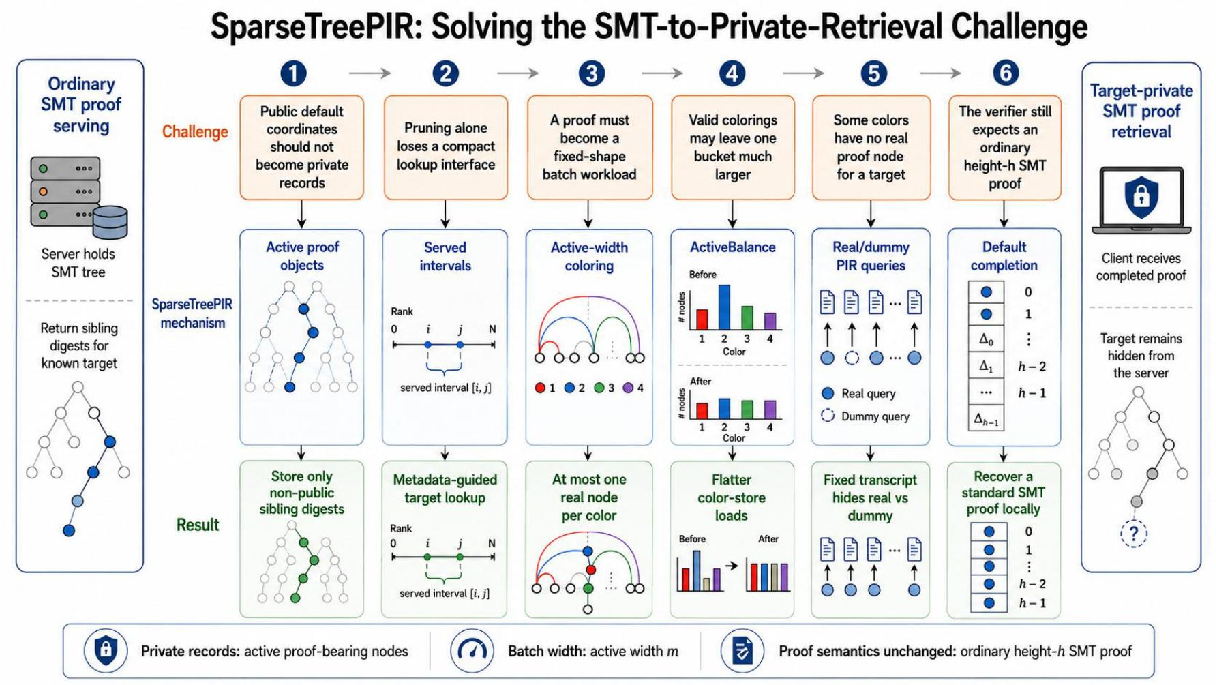
\includegraphics[width=0.98\textwidth]{../figures/sparsetreepir_private_retrieval_solution_figure.pdf}
\caption{SparseTreePIR solution map from ordinary SMT proof serving to target-private proof retrieval. The retrieval mechanism stores only non-default proof digests in color subdatabases, uses target-interval metadata for lookup, hides real and dummy PIR roles with a fixed query pattern, balances subdatabase sizes with \ActiveBalance{}, and reconstructs the standard height-$h$ SMT proof locally.}
\label{fig:algorithm-stack}
\end{figure*}

The rest of the paper is organized as follows. Section~\ref{sec:background} gives the background and problem setting needed for our formulation. Section~\ref{sec:related} positions SparseTreePIR relative to authenticated maps, TreePIR, and PIR backends. Section~\ref{sec:model} defines the problem, leakage model, and PIR-retrievable sibling nodes. Section~\ref{sec:coloring} presents the SparseTreePIR construction. Section~\ref{sec:correctness} proves correctness, target privacy, and complexity properties. Section~\ref{sec:experiments} evaluates the resulting private-retrieval layout and balancing algorithm. Section~\ref{sec:conclusion} concludes.

\section{Background and Problem Setting}
\label{sec:background}

This section reviews the background and problem setting needed for private retrieval of Sparse Merkle Tree (SMT) membership proofs. We use standard terminology where possible. The proof verified by the client remains a standard height-$h$ SMT membership proof: one sibling digest per level, checked against a public root. The database queried through PIR should contain only the non-default proof material that cannot be reconstructed from public default hashes. The client combines PIR-retrieved digests with the public default-hash chain before ordinary verification.

\subsection{Merkle Proof Retrieval}

A binary Merkle tree commits to a set of records by hashing the records at the leaves and recursively hashing pairs of child digests until a single root digest is obtained~\cite{merkle}. To verify membership of a target leaf, the verifier uses the leaf value and an authentication path consisting of one sibling digest at each level from the leaf to the root. The verifier recomputes the path upward and accepts if the resulting root equals the public commitment.

From a retrieval perspective, a Merkle authentication path is a path-dependent batch of records rather than a single database item. A direct proof request reveals the queried leaf: when the client asks the server for the proof of coordinate $i$, the server learns both $i$ and the corresponding path in the tree. PIR hides a selected database index, but applying PIR independently to every proof level ignores this path structure. TreePIR addresses the issue for perfect binary Merkle trees by partitioning proof nodes into color classes so that each proof path contains at most one node from each class, and the client sends one PIR query per class~\cite{treepir}. We follow the same path-aware batch-retrieval principle, but sparse SMTs require a different retrieval database.

\subsection{Sparse Merkle Proofs and Default Hashes}

A Sparse Merkle Tree is a Merkle tree over a fixed logical address space. A binary SMT of height $h$ has $2^h$ possible leaf coordinates, although only a subset of those coordinates may be occupied. Empty subtrees are represented by public default digests. Let $\Delta_0,\Delta_1,\ldots,\Delta_{h-1}$ denote the default-hash chain, where $\Delta_0$ is the digest of an empty leaf and $\Delta_{t+1}=H(\Delta_t\Vert \Delta_t)$. An empty sibling subtree of height $t$ therefore has digest $\Delta_t$.

An SMT membership proof for an occupied leaf still contains one sibling digest per level, so the proof length is always $h$. The important sparse-tree property is that some proof entries are public: if a sibling subtree is empty, the corresponding entry is the default digest for that level and does not need retrieval. If the sibling subtree is non-empty, its digest is a non-default sibling digest that may have to be obtained from the server. Thus the verification view is the standard height-$h$ membership proof, while the retrieval view contains only the non-default sibling digests that can appear in such proofs. The retrieval protocol changes how the proof is obtained, not how it is verified.

Figure~\ref{fig:smt-logical-storage} illustrates the two views of the same SMT snapshot. The verifier reasons about the full logical coordinate tree. The retrieval layer, however, should not materialize empty coordinates as PIR records: non-default nodes carry the only proof material that must be retrieved, while empty proof levels are filled from the public default-hash chain.

\begin{figure}[h]
	\centering
	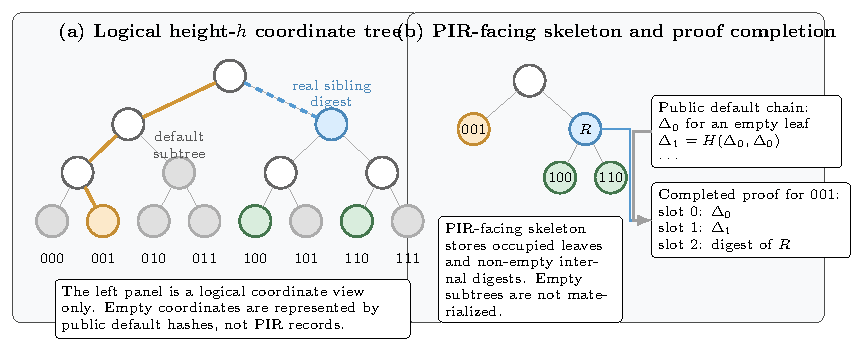
\includegraphics[width=\linewidth]{../figures/sparsetreepir_smt_logical_storage_figure.pdf}
	\caption{Logical and retrieval views of an SMT. The verifier reasons about a complete height-$h$ coordinate tree, but the PIR database should not store every empty coordinate. A membership proof is completed by combining PIR-retrieved non-default sibling digests with public default hashes.}
	\label{fig:smt-logical-storage}
\end{figure}

\subsection{From Proof Privacy to Batch PIR}

The privacy goal is query privacy for membership-proof retrieval: given a fixed public SMT snapshot, the server should not learn which occupied leaf the client is proving, nor which authentication path is selected. The tree root, the default-hash chain, and the public retrieval layout may be known to the server.

A simple solution would run one PIR query for every level of the height-$h$ proof. This hides the target, but it treats the proof as $h$ independent lookups and may issue unnecessary queries for levels whose sibling digests are public defaults. Generic batch-PIR schemes can retrieve multiple records privately, but they treat the requested records as an arbitrary batch. They do not specify which SMT proof records should be stored in the PIR database, how default proof entries should be omitted, or how the client should reconstruct the standard SMT proof after retrieval. The sparse setting therefore needs an SMT-specific retrieval layout: simply deleting empty records from a perfect-tree layout is not enough, because the remaining records must still be indexed, partitioned into subdatabases, queried with a fixed query pattern, and mapped back to the correct proof levels.

The construction in this paper stores only non-default sibling digests that may be required by some occupied-leaf membership proof. These records are partitioned into subdatabases so that, for any target, the client needs at most one real record from each subdatabase. The online protocol sends one PIR query to each subdatabase. If the target proof requires a record from that subdatabase, the query selects that record; otherwise, it is a dummy query sampled through the same PIR interface. The server observes a fixed-size batch of well-formed PIR queries, while the client locally determines which responses correspond to proof entries.

\subsection{Retrieval Workload Metrics}

We treat the underlying PIR scheme as a black-box backend. The contribution of the retrieval layout is therefore the database and query profile exposed to existing PIR schemes, rather than a new PIR primitive. For a fixed SMT snapshot, the main quantities are: (i) the number of non-default proof records stored in the PIR database; (ii) the number of PIR subqueries sent for one membership proof; (iii) the maximum subdatabase size; and (iv) the amount of public metadata needed for client-side lookup.

These quantities do not fully determine every PIR implementation's running time, because practical systems differ in packing methods, preprocessing, cryptographic parameters, and query/response formats~\cite{chor,ko97,xpir,sealpir,spiral,simplepir}. They do determine the structural workload given to the backend: sequential execution scales with the queried subdatabases, while parallel execution is often limited by the largest subdatabase. This resource view also clarifies the baseline. Once query privacy is required, the relevant comparison is not ordinary SMT proof serving, but privacy-preserving layouts that store different proof-record sets, issue different numbers of PIR subqueries, and expose different subdatabase sizes.

The resulting design problem is as follows. Given a fixed public SMT snapshot, determine which non-default sibling digests should be stored as PIR records, how these records should be partitioned into subdatabases, and how the client should reconstruct the standard height-$h$ SMT membership proof from PIR responses and public default hashes. Section~\ref{sec:model} formalizes the retrievable record set, the associated target intervals, and the leakage model. Section~\ref{sec:coloring} then presents the SparseTreePIR construction.

\section{Related Work}
\label{sec:related}

\textit{Merkle trees and authenticated data structures.}
Merkle's hash-tree construction~\cite{merkle} underlies authenticated dictionaries and generic authenticated data structures~\cite{padauth,adsgeneric}. Deployed systems use Merkle-style commitments for certificate-transparency logs~\cite{ctv2,ctqueue,crosbywallach}, key-transparency and verifiable-directory systems~\cite{coniks,transdict,parakeet,optiks}, replicated key-value stores~\cite{dynamo}, append-only authenticated structures~\cite{balloon}, and blockchain or stateless-client commitments~\cite{utreexo,ethereum,zcash}. These systems provide integrity and efficient verification, but they do not hide which proof a client requests. Our setting keeps the SMT snapshot and public metadata visible, while hiding the queried occupied leaf.

\textit{Sparse Merkle trees and proof generation.}
SMTs support large logical key spaces by assigning public default hashes to empty subtrees~\cite{sparsemt}. They appear in revocation/transparency maps, authenticated maps, constrained revocation checking, and state-commitment structures such as Jellyfish Merkle Tree~\cite{revtrans,vcer,jmt}. Recent work optimizes proof size, multiproofs, non-membership proofs, batch updates, or alternative authenticated structures~\cite{compactmultiproof,rollupsmt,multicollisiontree}. These systems improve ordinary SMT storage, updates, or proof generation. SparseTreePIR keeps the standard verification interface: the client reconstructs a height-$h$ membership proof. The change is at the retrieval layer, where only non-default sibling digests are queried through PIR and default-empty levels are reconstructed locally.

\begin{table*}[!t]
\centering
\caption{Representative authenticated-map and SMT proof-serving systems and their relation to private proof retrieval}
\label{tab:smt-prior-proof-serving}
\scriptsize
\setlength{\tabcolsep}{4pt}
\begin{tabular}{>{\raggedright\arraybackslash}p{0.19\textwidth}
                >{\raggedright\arraybackslash}p{0.34\textwidth}
                >{\raggedright\arraybackslash}p{0.17\textwidth}
                >{\raggedright\arraybackslash}p{0.22\textwidth}}
\toprule
Work & Reported goal/result & Optimized layer & Relation to our setting \\
\midrule
Efficient SMTs~\cite{sparsemt} &
Formal SMT operations and caching; audit paths for membership/non-membership can be generated in practically constant time, reported below $4$ ms with SHA-512/256 &
Plain proof generation &
Non-private lower bound: server knows the queried coordinate \\
\addlinespace
Jellyfish Merkle Tree~\cite{jmt} &
SMT variant for Diem state storage; optimizes node keys, node types, proof format, LSM-tree storage, I/O, and computation &
Deployed state-tree storage &
Representative SMT-system baseline, but proof requests are visible lookups \\
\addlinespace
Compact Merkle multiproofs~\cite{compactmultiproof} &
Sparse multiproof encoding keeps only $k$ leaf indices instead of an index for every non-leaf hash in a multiproof &
Multi-target proof compression &
Reduces proof payload for known targets; does not hide which targets are requested \\
\addlinespace
Rollup SMT batch update~\cite{rollupsmt} &
For zkSync Lite-style updates, improves account update time from $O(\log n)$ to $O(1)$ and reduces batch update cost by a one-pass traversal &
State update/root recomputation &
Orthogonal to retrieval privacy; update cost is not the bottleneck studied here \\
\addlinespace
Multicollision-resistant non-membership tree~\cite{multicollisiontree} &
Reduces authenticated (non-)membership tree depth for ZK-oriented settings while preserving security parameters &
Alternative accumulator/proof structure &
Changes the authenticated structure; our work keeps standard SMT proof semantics while privatizing retrieval \\
\bottomrule
\end{tabular}
\end{table*}

\textit{Private retrieval of authenticated proofs.}
Private retrieval of authenticated proofs has been studied in multi-client and transparency-log settings~\cite{lueksgoldberg,ctprivacy,kalesct}. The closest structural baseline is TreePIR~\cite{treepir}, which partitions proof nodes of a perfect binary Merkle tree into color classes so that each proof path contains at most one node from each class. SparseTreePIR uses the same one-query-per-color principle, but the database records are different. TreePIR is formulated for a perfect-tree proof layout; an SMT contains public default proof positions that should not be stored or queried through PIR. Pruning those records after expanding to a perfect tree still leaves the wrong query universe. SparseTreePIR instead builds the PIR database directly from non-default sibling digests that can occur in occupied-leaf membership proofs, uses interval metadata for lookup, and reconstructs the ordinary height-$h$ proof with default hashes. Thus it is an SMT proof-retrieval layout, not a new PIR primitive and not a direct TreePIR instantiation.

\textit{Batch PIR and practical PIR backends.}
PIR began with multi-server information-theoretic constructions~\cite{chor} and single-server computational PIR~\cite{ko97,cms}. Batch retrieval uses batch codes and combinatorial batch codes~\cite{batchcodes,cbc}; practical systems use probabilistic batch codes, Cuckoo-style placement, vectorized processing, or constant-weight-code techniques~\cite{sealpir,cuckoo,vectorbatchpir,pirana}. Backends such as XPIR, OnionPIR, Spiral, SimplePIR, PIANO, and YPIR improve communication, server computation, packing, and preprocessing~\cite{xpir,onionpir,spiral,simplepir,piano,ypir}. These systems provide the private-retrieval backend. They do not specify which SMT proof records should enter the PIR database, how to group them into subdatabases, or how to reconstruct the standard SMT proof. SparseTreePIR exposes such a database layout to any compatible backend; real and dummy queries are hidden by the query privacy of the underlying PIR scheme.

\textit{Baselines derived from prior work.}
Existing SMT systems optimize ordinary proof serving: the server traverses the requested coordinate and returns the sibling digests needed for verification~\cite{sparsemt,revtrans,vcer,jmt}. Some default-empty siblings can be omitted because the client reconstructs them from public defaults, but the request still reveals the key or path. Table~\ref{tab:prior-baselines} separates what each prior line provides from what remains missing for batch PIR. Once query privacy is required, the relevant comparison is between PIR database layouts for the same proof-retrieval task, rather than only against non-private proof-serving systems or internal ablations.

\begin{table*}[!t]
\centering
\caption{PIR database layouts for private SMT proof retrieval derived from prior work}
\label{tab:prior-baselines}
\scriptsize
\setlength{\tabcolsep}{4pt}
\begin{tabular}{>{\raggedright\arraybackslash}p{0.18\textwidth}
                >{\raggedright\arraybackslash}p{0.26\textwidth}
                >{\raggedright\arraybackslash}p{0.20\textwidth}
                >{\raggedright\arraybackslash}p{0.27\textwidth}}
\toprule
Prior line & Natural proof object & Induced baseline & Missing for our goal \\
\midrule
Standard SMT proof APIs~\cite{sparsemt,revtrans,jmt} &
Height-$h$ proof path with non-default siblings and public defaults &
Plain SMT proof serving &
No target privacy; server sees the queried coordinate/path \\
\addlinespace
Compact SMT storage~\cite{sparsemt,vcer,jmt} &
Non-default skeleton plus public default chain &
Non-default proof-record serving &
Saves storage, but gives no fixed PIR query pattern \\
\addlinespace
Generic batch-PIR placement~\cite{batchcodes,cbc,sealpir} &
Non-default proof records treated as an arbitrary batch &
PBC-style SMT; unpartitioned active-record PIR &
Ignores ancestor/path structure; may query or replicate too much \\
\addlinespace
TreePIR on perfect trees~\cite{treepir} &
Colored proof nodes in a perfect-tree layout &
Complete-tree and height-preserving pruned TreePIR &
Colors the full coordinate tree, including public default positions \\
\addlinespace
This paper &
Non-default sibling digests with interval metadata &
SparseTreePIR &
Fixed-pattern batch PIR with local default-hash reconstruction \\
\bottomrule
\end{tabular}
\end{table*}

\textit{Balancing color subdatabases.}
A valid coloring does not necessarily give an efficient PIR layout: one color subdatabase may be much larger than the others. Perfect-tree coloring reduces the number of queries for perfect Merkle trees, but it does not address the load imbalance caused by sparse SMT snapshots. \ActiveBalance{} is a backend-independent refinement that preserves the same fixed number of PIR queries while reducing the largest queried subdatabase, complementing ordinary SMT proof-generation optimizations.

\section{Problem Formulation and Leakage Model}
\label{sec:model}

This section formalizes the private retrieval problem studied in this paper. We consider a fixed public snapshot of a binary Sparse Merkle Tree (SMT). The tree height, root commitment, occupied-leaf set, public default-hash chain, and the PIR database layout produced during setup are treated as public snapshot information. The privacy goal is query privacy within this fixed snapshot: during online retrieval, the storage server should not learn which occupied leaf is queried, which non-default sibling digests are needed for its proof, or which PIR queries are real rather than dummy queries.

The formal model targets membership-proof retrieval for occupied leaves. Non-membership retrieval over absent coordinates is a natural extension, but it changes the query domain from the public occupied-leaf set to the full logical address space. It also requires metadata for absent coordinate regions and an explicit leakage choice about whether the server learns that the query is a non-membership query. We therefore leave non-membership privacy outside the present model.

A PIR record in this paper means a database record that is retrieved through PIR because it cannot be reconstructed from public default hashes. The record content itself is not assumed to be hidden from the storage server. The protected information is the selected index, or equivalently the queried target leaf, relative to the setup leakage defined below.

\subsection{Fixed-Snapshot Proof Records}

Let $T$ be a fixed binary Sparse Merkle Tree of height $h$, and let $\mathcal{L}$ denote its set of occupied leaves. Hashes are still computed in the standard bottom-up way. The retrieval layout introduced below does not change the SMT hash construction; it only specifies which proof digests are placed in PIR subdatabases. We assume the standard public default-hash chain
\[
\Delta_0,\Delta_1,\ldots,\Delta_{h-1},
\]
where $\Delta_0$ is the default empty-leaf digest and $\Delta_{t+1}=H(\Delta_t\Vert \Delta_t)$ for $0\le t<h-1$. Thus, every empty sibling subtree of height $t$ has publicly reconstructible digest $\Delta_t$.

\begin{definition}[PIR-retrievable sibling node]
For a node $u$ in $T$, let $\operatorname{cnt}(u)$ be the number of occupied leaves in the subtree rooted at $u$. Let $u$ be a non-root node, and let $\operatorname{sib}(u)$ be its sibling. We say that $u$ is a \emph{PIR-retrievable sibling node} if
\[
\operatorname{cnt}(u)>0
\qquad\text{and}\qquad
\operatorname{cnt}(\operatorname{sib}(u))>0.
\]
The set of all PIR-retrievable sibling nodes is denoted by $\mathcal{A}(T)$.
\end{definition}

The first condition ensures that $u$ itself has a non-default digest. The second condition ensures that $u$ can appear as a sibling node in the membership proof of at least one occupied target leaf. Thus $\mathcal{A}(T)$ contains exactly the non-default sibling digests that may have to be retrieved through PIR. Empty sibling subtrees remain outside the PIR database because their digests are publicly reconstructible from the default-hash chain.

\begin{proposition}[Minimal non-default PIR record set]
\label{prop:active-record-minimality}
Fix a public height-$h$ SMT snapshot $T$ and the public default-hash chain, and assume the SMT hash function is collision resistant. In the record-based retrieval model where a PIR record supplies one proof sibling digest and public default values are filled locally, $\mathcal{A}(T)$ is exactly the set of non-default sibling digests that may be required by some occupied-leaf membership proof, except with negligible hash-collision probability. Consequently, any PIR database that supports all occupied-leaf membership proofs must make one digest for every node in $\mathcal{A}(T)$ retrievable, while no default-empty sibling position needs a PIR record.
\end{proposition}

\begin{proof}
If $u\in\mathcal{A}(T)$, then $u$ is non-empty and $\operatorname{sib}(u)$ is also non-empty. Choose any occupied leaf in the subtree of $\operatorname{sib}(u)$; the standard membership proof for that leaf contains the digest of $u$ as a sibling digest. By collision resistance, a non-empty subtree digest is computationally distinct from the corresponding public default digest except with negligible probability. Thus a record-based private retrieval layout that reconstructs every occupied-leaf proof must make this digest retrievable. Conversely, if a proof sibling subtree is empty, its digest is the public value $\Delta_t$ for the corresponding height $t$ and is reconstructed locally. A non-empty node whose sibling subtree is empty is not a sibling for any occupied target leaf. Therefore the necessary and sufficient non-default PIR record set is precisely $\mathcal{A}(T)$.
\end{proof}

\begin{definition}[PIR-retrievable sibling set]
For any occupied leaf $\ell \in \mathcal{L}$, let
\[
\mathsf{Path}(\ell)\subseteq \mathcal{A}(T)
\]
denote the sequence of all PIR-retrievable sibling nodes in the standard Merkle proof of $\ell$, ordered from higher to lower proof levels.
\end{definition}

Equivalently, $\mathsf{Path}(\ell)$ contains exactly those sibling nodes on the standard height-$h$ proof of $\ell$ whose subtrees contain at least one occupied leaf. Sibling levels whose subtrees are empty are not PIR records and are later filled locally with the corresponding default hash.

Although the full SMT proof length is always $h$, the number of PIR records in $\mathsf{Path}(\ell)$ may be smaller than $h$, because some levels correspond only to publicly reconstructible default-empty nodes.

Let
\[
m=\max_{\ell\in\mathcal{L}} |\mathsf{Path}(\ell)|
\]
be the \emph{retrieval width} of the snapshot, namely the maximum number of non-default sibling digests that can appear in one occupied-leaf membership proof. Equivalently, this is the active width used by SparseTreePIR. By construction, $m\le h$. Once the PIR-retrievable record set is fixed, this same quantity is also the number of color classes and the batch width of the one-query-per-color retrieval layout. Throughout the paper, $[m]$ denotes $\{1,\ldots,m\}$.

The case $|\mathcal{L}|=1$ is degenerate: no occupied target has a non-default sibling subtree, so $\mathcal{A}(T)=\emptyset$, $m=0$, and no PIR query is issued. Unless explicitly stated otherwise, the rest of the paper assumes $|\mathcal{L}|\ge 2$.

The role of $m$ is analogous to the role of $h$ in TreePIR only after public default-empty levels have been removed from the PIR database layout. It is not a tunable parameter chosen by the balancing algorithm; it is a public resource parameter of the fixed SMT snapshot. The verifier still receives a height-$h$ proof after client-side reconstruction. The retrieval width only measures how many proof positions may require private retrieval under the record-based retrieval model.

\begin{remark}[Why $m$ can be much smaller than $h$]
The value of $m$ is necessarily instance-dependent because it depends on where the occupied leaves branch. The setup phase publishes $m$ as part of the public layout, just as a perfect-tree TreePIR setup publishes height $h$. To interpret this parameter, suppose $n$ occupied leaves are sampled uniformly from a logical universe of size $U=2^h$, and condition on one target leaf. At proof level $t$ above the leaf, the sibling subtree contains $2^t$ logical leaves, so the probability that this level contributes a non-default sibling digest is
\[
1-\frac{\binom{U-1-2^t}{n-1}}{\binom{U-1}{n-1}}
\approx 1-\exp\!\left(-\frac{(n-1)2^t}{U-1}\right).
\]
Thus the expected number of PIR-retrievable proof positions for a random target is the sum of these probabilities over $t=0,\ldots,h-1$. When $n\ll U$, most low levels have empty sibling subtrees and only the levels near the branching depth of the occupied set contribute; the retrieval width therefore tracks the branching structure of the occupied leaves rather than the logical height. In adversarial layouts, the sharp worst-case bound remains $m\le\min\{h,n-1\}$.
\end{remark}

This paper focuses on target-private retrieval of \emph{membership} proofs for occupied leaves in a fixed public SMT snapshot. This scope matches the proof-retrieval setting in which the client privately asks for the authentication material of an existing committed object. Non-membership retrieval is a natural extension, but it changes the object being hidden. The target domain becomes the full logical coordinate space rather than the public occupied-leaf set; a proof may certify an empty coordinate, a divergence from the nearest occupied prefix, or a gap between existing keys; and the protocol must specify whether the server should learn that the query is for an absent coordinate. Consequently, the interval metadata would have to range over logical coordinates or absent-coordinate regions, not only over occupied-leaf ranks. We therefore keep non-membership SparseTreePIR outside the present formal model and treat it as a separate extension requiring its own metadata and leakage model.

\subsection{Target-Rank Intervals}

To support efficient indexing, we associate each PIR-retrievable sibling node with the interval of target leaves for which it acts as a proof sibling. This is not the subtree interval of $u$ itself. Order the occupied leaves by their logical SMT positions and let $r(\ell)\in\{0,\ldots,|\mathcal{L}|-1\}$ be the occupied-leaf rank of $\ell$. Let $s=\operatorname{sib}(u)$, and define the \emph{target-rank interval}
\[
I_{\mathsf{srv}}(u) = [L(s),R(s)]
\]
as the interval of occupied-leaf ranks covered by the sibling subtree of $u$. Thus $L(s)$ and $R(s)$ are rank endpoints, not heap-index endpoints in the full logical coordinate space. Then, for any occupied leaf $\ell$,
\[
u \in \mathsf{Path}(\ell) \Longleftrightarrow r(\ell) \in I_{\mathsf{srv}}(u).
\]

Since every binary subtree corresponds to a contiguous interval in leaf order, the resulting target-rank intervals form a laminar family: any two intervals are either disjoint, or one contains the other. This structure underlies both the coloring method and the indexing method.

\subsection{Coloring and Load Metrics}

The constructions below use $m$ color classes, where $m$ is the retrieval width defined above. Since $m\le h$, the resulting batch profile is no wider than the SMT verifier height. Section~\ref{sec:correctness} later states the corresponding model-specific lower-bound argument: under the one-query-per-color model, a proof requiring $m$ PIR records needs $m$ distinct colors.

\begin{definition}[Proper coloring]
A map
\[
\varphi:\mathcal{A}(T)\rightarrow[m]
\]
is a \emph{proper coloring} if for every occupied leaf $\ell\in\mathcal{L}$ and every two distinct nodes $u,v\in\mathsf{Path}(\ell)$, we have
\[
u\neq v \Longrightarrow \varphi(u)\neq \varphi(v).
\]
\end{definition}

A proper coloring ensures that every membership proof needs at most one real PIR record from each color subdatabase.

For a color $c\in[m]$, let
\[
\mathcal{D}_c=\{u\in\mathcal{A}(T): \varphi(u)=c\}
\]
be the corresponding color subdatabase, with size $N_c=|\mathcal{D}_c|$. Let $N=|\mathcal{A}(T)|$, and let
\[
\overline{N}=N/m
\]
be the average subdatabase size. The main optimization target in this paper is to keep the color subdatabases as balanced as possible while preserving proper coloring. In particular, we track
\[
M(\varphi)=\max_c N_c,
\qquad
\Delta_N(\varphi)=\max_c N_c-\min_c N_c,
\]
and the normalized maximum-subdatabase ratio
\[
R(\varphi)=\frac{M(\varphi)}{\overline{N}}.
\]
Here $M(\varphi)$ is the direct structural bottleneck, while $\Delta_N(\varphi)$ and $R(\varphi)$ indicate how far the partition is from an equal split.

The \ActiveBalance{} scheme is self-contained. It first constructs a feasible coloring by a first-fit traversal of the laminar interval forest, and then refines that coloring by subtree-level color permutations that directly improve the global subdatabase loads.

\begin{definition}[Client-side inputs and public metadata]
For a target leaf $\ell$, the client uses the following local inputs and public metadata before issuing PIR queries:
\begin{enumerate}[leftmargin=2em]
  \item the tree height $h$ and the position of $\ell$ in the SMT;
  \item the default-hash chain $\Delta_0,\ldots,\Delta_{h-1}$;
  \item the occupied-leaf rank $r(\ell)$ of the target within the public ordered set of occupied leaves;
  \item for each color $c\in[m]$, a public metadata table
  \[
  \mathcal{M}_c=\bigl((I_{\mathsf{srv}}(u),\delta(u))\bigr)_{u\in\mathcal{D}_c},
  \]
  sorted by interval, where the two endpoints of $I_{\mathsf{srv}}(u)$ are occupied-leaf ranks and $\delta(u)=h-\operatorname{depth}(u)$ denotes the proof level of $u$ measured from leaf to root.
\end{enumerate}
\end{definition}

The PIR subdatabases store node digests. The level and interval information required for client-side proof reconstruction is carried by the public metadata tables rather than by PIR records.

\subsection{Setup Leakage and Target Privacy}

The retrieval protocol in this paper hides the queried target leaf inside one \emph{fixed public SMT instance}; it does not aim to hide the entire occupancy pattern of that instance. We model the storage server's snapshot-level view with the following deterministic setup leakage.

\begin{definition}[Setup leakage]
\label{def:leakagefunction}
Let setup on a fixed SMT snapshot $T$ produce retrieval width $m$, PIR-retrievable node set $\mathcal{A}(T)$, coloring $\varphi:\mathcal{A}(T)\to[m]$, color subdatabases $\{\mathcal{D}_c\}_{c=1}^{m}$, and public metadata tables $\{\mathcal{M}_c\}_{c=1}^{m}$. Let $N_c=|\mathcal{D}_c|$. The setup leakage visible to the storage server is
\[
\begin{aligned}
\mathcal{L}_{\mathsf{setup}}(T)=
\Bigl(&h,\mathsf{root}(T),\mathcal{L},
\{\Delta_t\}_{t=0}^{h-1},\\
&\mathcal{A}(T),m,\varphi,
\{(\mathcal{D}_c,\mathcal{M}_c,N_c)\}_{c=1}^{m}
\Bigr).
\end{aligned}
\]
Thus the leakage includes the fixed occupancy pattern, the committed root, the public default-hash chain, the PIR-retrievable node set, the coloring, the color subdatabases, the public metadata, and the subdatabase sizes. For an online target $\ell$, it does not include $\ell$, the set $\mathsf{Path}(\ell)$ of required PIR records, the set of colors containing real proof records, or the selected item index inside any color subdatabase. The only target-independent online shape revealed by the protocol is that every retrieval sends exactly one PIR subquery to each of the $m$ color subdatabases.
\end{definition}

The hidden query information consists of the target leaf $\ell$, equivalently the required PIR record set $\mathsf{Path}(\ell)$, as well as which color positions correspond to real retrievals rather than dummy subqueries and which item index is privately selected inside each color subdatabase.

\begin{table}[t]
\centering
\caption{Server-visible setup state and hidden query information}
\label{tab:leakage}
\scriptsize
\setlength{\tabcolsep}{4pt}
\begin{tabular}{>{\raggedright\arraybackslash}p{0.45\linewidth}>{\raggedright\arraybackslash}p{0.45\linewidth}}
\toprule
Visible to the storage server & Hidden by PIR queries \\
\midrule
root, occupied-leaf set, default-hash chain, PIR-retrievable node set, color subdatabases, interval metadata, color assignment, subdatabase sizes, retrieval width $m$
&
target leaf $\ell$, required PIR records, which color slots are real or dummy, selected item index inside each color subdatabase \\
\bottomrule
\end{tabular}
\end{table}

We make this leakage profile explicit. The retrieval layout is precomputed once for a fixed SMT snapshot and is treated as server-visible structure thereafter. Our privacy claim is therefore \emph{query privacy relative to a server-visible PIR database layout}, rather than structure privacy for the whole sparse tree. The corresponding transcript view has a fixed query shape: the server sees one well-formed PIR query per color, while the real/dummy roles are client-local.

\begin{definition}[Target privacy game]
\label{def:privacygame}
Let $\mathcal{L}_{\mathsf{setup}}(T)$ be the setup leakage in Definition~\ref{def:leakagefunction}. In the experiment $\mathsf{PrivTarget}_{\mathcal{A}}(\lambda)$, the challenger runs setup for the fixed SMT snapshot and gives $\mathcal{L}_{\mathsf{setup}}(T)$ to the adversary $\mathcal{A}$. The adversary chooses two occupied target leaves $\ell_0,\ell_1\in\mathcal{L}$. The challenger samples $b\leftarrow\{0,1\}$, runs the batch query-generation algorithm for $\ell_b$, and gives the full batch query transcript to $\mathcal{A}$. The adversary outputs a bit $b'$. Its advantage is
\[
\operatorname{Adv}^{\mathsf{target}}_{\mathcal{A}}
=\left|\Pr[b'=b]-\frac12\right|.
\]
The protocol is target-private relative to $\mathcal{L}_{\mathsf{setup}}(T)$ if this advantage is negligible for every efficient adversary.
\end{definition}

For dummy positions, the client samples a well-formed PIR query to a valid index in the same color subdatabase, independently of the target leaf, and discards the response. The setup layout exposes only non-empty color subdatabases. Implementations that allow empty color classes can remove them during setup or pad them with one public dummy record.

\section{SparseTreePIR Construction}
\label{sec:coloring}

This section presents the fixed-snapshot retrieval protocol. Offline preprocessing constructs the PIR database from the compressed non-default SMT representation, rather than from a materialized full binary tree. Online retrieval issues a target-independent batch of PIR queries and reconstructs the standard height-$h$ SMT membership proof locally using public default hashes.

\subsection{Construction Overview}

SparseTreePIR instantiates a snapshot-specific retrieval layout with a target-independent online transcript. During setup, the server identifies active proof records, partitions them into color subdatabases, and publishes metadata that maps target ranks to lookup intervals. During online retrieval, the client sends exactly one PIR subquery to each color subdatabase. If the target proof needs a record in that color, the query selects that record. Otherwise, the query is a dummy sampled through the same PIR interface. After receiving the responses, the client writes the real digests into the appropriate proof slots and fills the remaining slots with public default hashes. Figure~\ref{fig:workflow} summarizes this setup-and-retrieval flow.

\begin{figure}[!t]
	\centering
	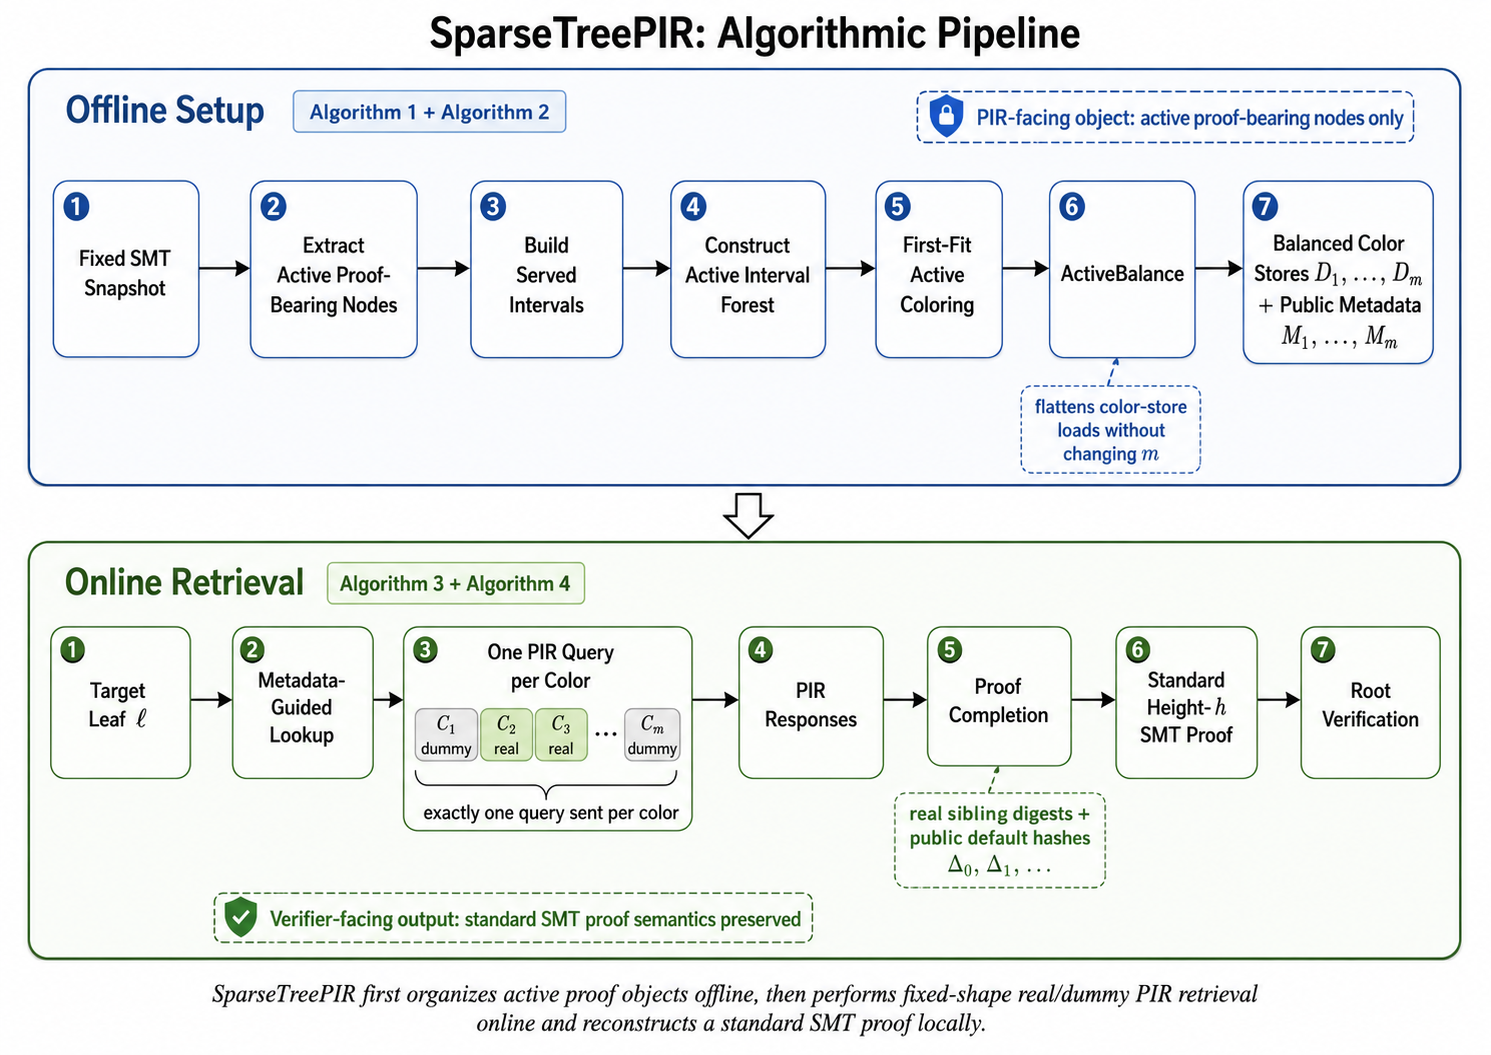
\includegraphics[width=\linewidth]{../figures/sparsetreepir_algorithmic_pipeline.png}
	\caption{SparseTreePIR algorithmic pipeline. Offline setup extracts active proof records, builds target-rank intervals, colors the laminar interval forest, and balances color subdatabases. Online retrieval uses public metadata to issue exactly one PIR query per color, then combines retrieved non-default sibling digests with public default hashes to reconstruct the standard height-$h$ SMT proof.}
	\label{fig:workflow}
\end{figure}

\noindent\textbf{Online retrieval pattern.}
Given a fixed public SMT snapshot $T$, setup outputs color subdatabases
$\mathcal{D}_1,\ldots,\mathcal{D}_m$, public metadata tables
$\mathcal{M}_1,\ldots,\mathcal{M}_m$, and $m$ color classes. For every occupied target leaf, the client sends exactly one PIR subquery to each $\mathcal{D}_c$. A subquery is real if color $c$ contains the non-default sibling digest required by the target proof, and dummy otherwise. The client then combines the real PIR outputs with the public default-empty hash chain to reconstruct the standard height-$h$ SMT proof. The PIR workload metrics are storage $|\mathcal{A}(T)|$, retrieval width $m$, largest subdatabase size $\max_c|\mathcal{D}_c|$, and public metadata size $O(|\mathcal{A}(T)|)$.

The algorithms below are presented as a protocol stack rather than as independent routines. Algorithm~\ref{alg:color} is the server-side setup procedure for one fixed public SMT snapshot. It extracts active proof records, computes the retrieval-width parameter, invokes Algorithm~\ref{alg:activebalance} as a balancing subroutine, and publishes the metadata consumed by the client. Algorithm~\ref{alg:query} is the online client lookup and query-generation procedure. It consumes exactly the public outputs of setup and produces two outputs: the batch of PIR subqueries sent to the server, and a client-side selection map that is never revealed. After the underlying PIR backend returns one response per color, Algorithm~\ref{alg:complete} uses that selection map, the public metadata, and the default-empty hash chain to reconstruct the standard height-$h$ SMT proof.

This separation mirrors the presentation style of TreePIR: setup fixes the colored database layout once, and every online retrieval has the same external profile. The server observes one PIR query per color subdatabase. Only the client knows which queries retrieve proof records and which are dummy queries.

\subsection{Running Example}

Figure~\ref{fig:smt-overview} presents the running example used in this section. It shows a complete height-$4$ coordinate tree for explanation, but the implementation traverses the compressed non-default representation and stores only active proof records in color subdatabases. Because the model has already defined the record set, target-rank intervals, and valid coloring, the example can now be interpreted as an instance of the formal interface rather than as an additional rule.

\begin{figure}[h]
\centering
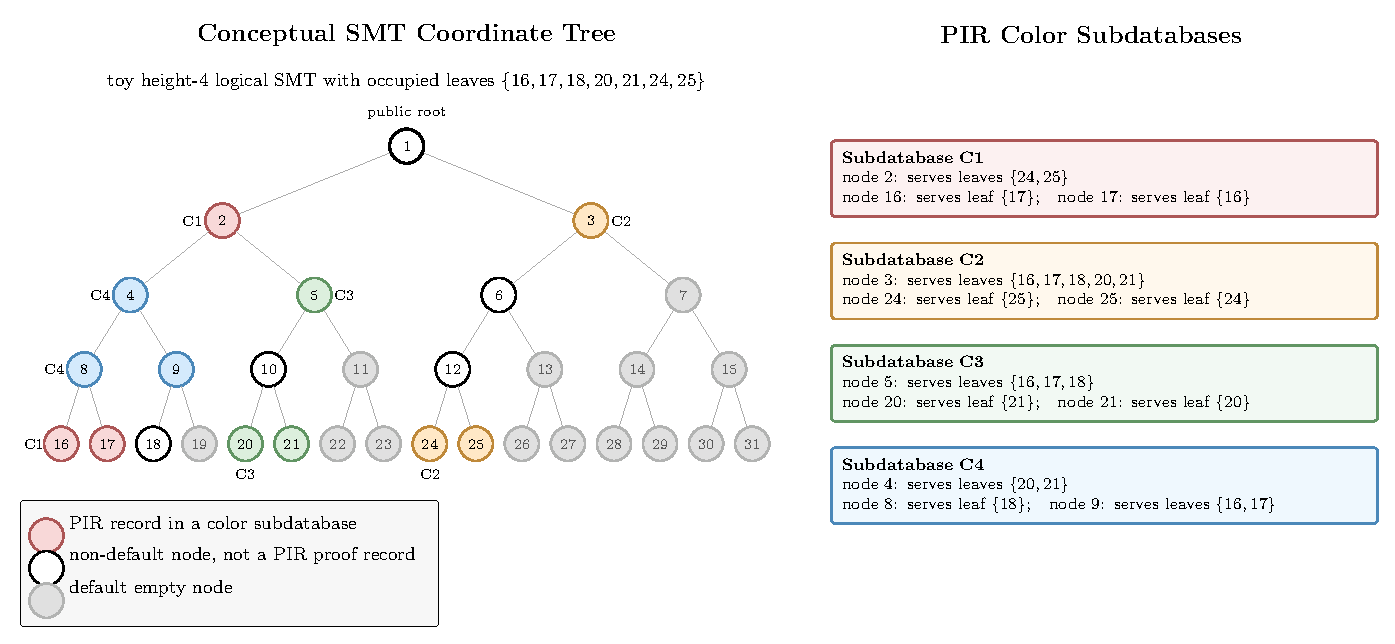
\includegraphics[width=\linewidth]{../figures/sparsetreepir_running_example_figure.pdf}
\caption{Running SMT example and its final color subdatabases. The full coordinate tree is explanatory; only active proof records are stored in PIR subdatabases.}
\label{fig:smt-overview}
\end{figure}

The example separates three standard objects. The first is the \emph{full SMT coordinate tree}, which determines hash positions and proof levels. The second is the set of non-default sibling digests that may appear in membership proofs; these digests form the active proof records stored in the PIR database. The third is \emph{client-side proof reconstruction}: proof levels whose sibling subtrees are empty are filled with public default hashes rather than retrieved through PIR. The figure labels intervals using logical leaf identifiers for readability; the actual public metadata stores target-rank intervals over the ordered occupied leaves.

The occupied leaves are $\{16,17,18,20,21,24,25\}$. The active proof records are exactly the twelve nodes shown in the color subdatabases of Figure~\ref{fig:smt-overview}:
\[
\{2,3,4,5,8,9,16,17,20,21,24,25\}.
\]
The longest PIR-retrievable sibling set has size $4$, so the setup exposes four color classes in this example.

This instance is useful because it already exhibits the balance problem. The first-fit feasibility stage may produce the legal color split
\[
\begin{aligned}
\mathcal{D}_1&=\{3,2\},\qquad
\mathcal{D}_2=\{5,4,25,24\},\\
\mathcal{D}_3&=\{9,8,21,20\},\qquad
\mathcal{D}_4=\{17,16\},
\end{aligned}
\]
whose subdatabase sizes are $(2,4,4,2)$. The coloring is valid but imbalanced. By contrast, subtree recoloring can transform the same interval forest into
\[
\begin{aligned}
\mathcal{D}_1&=\{2,17,16\},\qquad
\mathcal{D}_2=\{3,25,24\},\\
\mathcal{D}_3&=\{5,21,20\},\qquad
\mathcal{D}_4=\{4,9,8\},
\end{aligned}
\]
which is still valid and now has balanced subdatabase sizes $(3,3,3,3)$. This final split is deliberately not a layer coloring: for example, nodes $4$, $8$, and $9$ share color $4$ even though they lie at different logical depths in the full coordinate tree, while depth-$1$ nodes $2$ and $3$ have different colors. This is possible because the constraint is induced by target-rank intervals, not by raw tree depth. Figure~\ref{fig:beforeafter} visualizes this change. In the current algorithm, this improvement is reached by a short sequence of accepted legal subtree recolorings; the online query pattern stays fixed throughout. We will reuse the same small instance again when illustrating one concrete query and client-side proof reconstruction.

\begin{figure}[h]
\centering
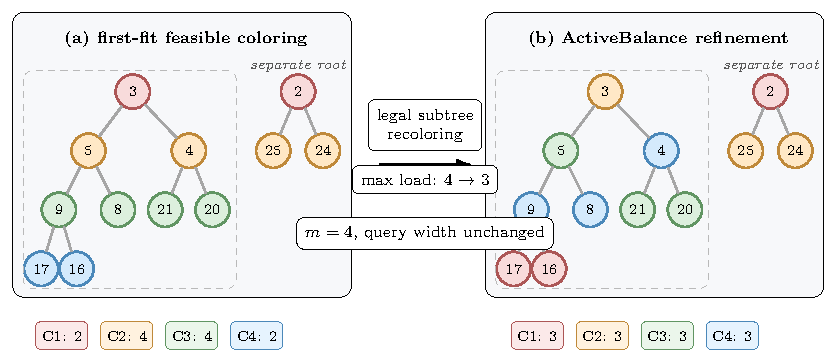
\includegraphics[width=\linewidth]{../figures/sparsetreepir_active_balance_before_after_figure.pdf}
\caption{Running example for the coloring stage. The first-fit feasibility stage leaves an uneven but valid split, while \ActiveBalance{} applies accepted legal subtree recolorings and reaches a flatter partition on the same interval forest.}
\label{fig:beforeafter}
\end{figure}

\subsection{Offline Preprocessing}

The preprocessing algorithm is run once for a fixed public SMT snapshot. It takes the occupied leaf set and the compressed non-default SMT representation as input, and outputs the color subdatabases and public metadata used by online retrieval. It does not materialize the full logical tree. Instead, it traverses the compressed non-default structure, identifies the non-default sibling digests that may appear in membership proofs, and records for each digest its target-rank interval and proof level. The resulting intervals form a laminar interval forest. Setup then computes a valid coloring, applies \ActiveBalance{} to reduce the largest subdatabase size, and publishes the metadata tables.

\begin{algorithm}[H]
\footnotesize
\caption{Offline preprocessing}
\label{alg:color}
\begin{algorithmic}[1]
\Require Fixed public SMT snapshot $T$, occupied leaf set $\mathcal{L}$, balancing rounds $R_1$
\Ensure Active width $m$, color subdatabases $\{\mathcal{D}_c\}_{c=1}^{m}$, public metadata tables $\{\mathcal{M}_c\}_{c=1}^{m}$, valid coloring $\varphi$
\State Sort the occupied leaves by logical SMT position and assign occupied-leaf ranks $0,\ldots,|\mathcal{L}|-1$
\State Build the compressed non-default skeleton $\mathcal{S}(T)$ induced by the occupied leaves
\State Annotate each skeleton edge with its corresponding original SMT child root and skipped logical levels
\State Initialize $\mathcal{A}(T)\gets \emptyset$
\For{each branching skeleton node $p$ with two non-default original children}
  \For{each original child root $u$ of $p$}
    \State $s \gets \operatorname{sib}(u)$ in the full SMT coordinate system
    \State Add $u$ to $\mathcal{A}(T)$
    \State Assign target-rank interval $I_{\mathsf{srv}}(u)=[L(s),R(s)]$ and proof level $\delta(u)$
  \EndFor
\EndFor
\State Sort all target-rank intervals by increasing left endpoint and decreasing interval length
\State Build the interval forest $\mathcal{F}$ from interval-containment relations
\State Set $m$ to the maximum depth of $\mathcal{F}$
\State Compute $\varphi\gets \textsc{FirstFitColoring}(\mathcal{F},m)$
\State Refine $\varphi\gets\ActiveBalance{}(\mathcal{F},\varphi,R_1)$ using Algorithm~\ref{alg:activebalance}
\State Build the color subdatabases $\mathcal{D}_c$ and the public metadata tables $\mathcal{M}_c$
\State \Return $m$, $\{\mathcal{D}_c\}_{c=1}^{m}$, $\{\mathcal{M}_c\}_{c=1}^{m}$, $\varphi$
\end{algorithmic}
\end{algorithm}

The first-fit stage is only a feasibility step. It traverses each tree of $\mathcal{F}$ from root to leaves and assigns every node the smallest color in $[m]$ not used on its strict ancestor chain. Since no target proof requires more than $m$ PIR records, such a color always exists. The actual balancing contribution is the subsequent \ActiveBalance{} recoloring step. The protocol-complete formulation remains specific to fixed binary SMTs, because client-side proof reconstruction relies on the standard default-empty hash chain.

From a systems viewpoint, Algorithm~\ref{alg:color} is the offline setup stage of the construction. Once the color subdatabases and public metadata tables have been built for one fixed SMT instance, the online retrieval protocol never needs to see the whole tree again. The expensive structural work is pushed offline, while the online stage sees only interval tables, color subdatabases, and the public default-hash chain.

\subsection{\ActiveBalance{}: Load Balancing by Subtree Recoloring}

A valid coloring guarantees that each proof needs at most one real record from each color subdatabase, but it does not guarantee balanced subdatabase sizes. A highly imbalanced coloring can make one PIR query much more expensive than the others. \ActiveBalance{} is a load-balancing procedure that preserves the retrieval width $m$ and changes only the assignment of records to colors. It evaluates subtree recolorings using the lexicographic load vector
\[
\Psi(\varphi)=
\operatorname{sort}_{\downarrow}(N_1,\ldots,N_m),
\]
so the objective is to reduce the largest subdatabase first and then flatten the remaining count vector.

For a rooted subtree $U$ of the interval forest and a color $c\in[m]$, let $C_U(c)$ denote the number of nodes of color $c$ currently appearing inside $U$. Let $A(U)\subseteq[m]$ be the set of colors not used on the strict ancestor chain of $U$. Since every node in $U$ must already be colored from $A(U)$, any permutation $\pi_U$ of these available colors can be applied uniformly inside $U$ without violating the coloring constraint. Proposition~\ref{prop:permvalid} shows that every such permutation preserves validity.

\begin{algorithm}[!t]
	\footnotesize
		\caption{\ActiveBalance{} subtree recoloring}
	\label{alg:activebalance}
	\begin{algorithmic}[1]
		\Require Laminar interval forest $\mathcal{F}$, valid coloring $\varphi$, rounds $R_1$
		\Ensure Updated valid coloring $\varphi$
		\State Compute global loads $\{N_c\}_{c=1}^{m}$ and $\Psi^\star\gets\Psi(\varphi)$
		\For{$t=1$ \textbf{to} $R_1$}
		\State Annotate each subtree root $U$ with ancestor colors and histogram $\{C_U(c)\}_{c=1}^{m}$
		\State $\mathsf{best}\gets\textsc{None}$
		\For{each subtree root $U$ in $\mathcal{F}$}
		\State $A(U)\gets [m]\setminus\text{AncestorColors}(U)$
		\If{$|A(U)|\le 1$} \State \textbf{continue} \EndIf
		\State Build $K_U[a,b]=(N_b-C_U(b)+C_U(a))^2$ for $a,b\in A(U)$
		\State Let $\pi_U$ be the min-cost perfect matching on $K_U$
		\State Form $\varphi'$ by applying $\pi_U$ inside $U$ and leaving all nodes outside $U$ unchanged
		\If{$\Psi(\varphi')<\Psi^\star$}
		\State $(\mathsf{best},\Psi^\star)\gets ((U,\pi_U,\varphi'),\Psi(\varphi'))$
		\EndIf
		\EndFor
		\If{$\mathsf{best}=\textsc{None}$} \State \textbf{break} \EndIf
		\State Apply $\mathsf{best}$ and update $\varphi$, $\{N_c\}_{c=1}^{m}$, and $\Psi^\star$
		\EndFor
		\State \Return $\varphi$
	\end{algorithmic}
\end{algorithm}

Algorithm~\ref{alg:activebalance} makes two design choices explicit. First, each subtree is evaluated against a count-only quadratic assignment objective rather than against the full combinatorial search over all possible recolorings. The cost term $(N_b-C_U(b)+C_U(a))^2$ is the squared size of subdatabase $b$ after the portion of color $b$ currently inside $U$ is removed and the portion of local color $a$ is mapped into it. Thus the surrogate favors moving heavier local color mass toward lighter global subdatabases. Second, after solving that local assignment, we accept a move only if the true global signature $\Psi(\varphi)$ decreases. Hence the surrogate guides the search, while the lexicographic load vector remains the actual acceptance rule.


\subsection{Target-Independent Online Query Generation}

After preprocessing, the client uses only public metadata to determine which color subdatabases contain proof records for the target. For each color $c$, the metadata table $\mathcal{M}_c$ is sorted by target-rank interval. Since intervals with the same color are disjoint, one binary search returns either a unique matching record or no matching record.

\begin{algorithm}[H]
\caption{Online query generation: one PIR subquery per color}
\label{alg:query}
\begin{algorithmic}[1]
\Require Target leaf $\ell$ with occupied-leaf rank $r(\ell)$, color subdatabases $\{\mathcal{D}_c\}_{c=1}^{m}$, public metadata tables $\{\mathcal{M}_c\}_{c=1}^{m}$, underlying PIR query generator $\mathsf{PIR.Query}$
\Ensure Batch query $\mathcal{Q}=\{Q_c\}_{c=1}^{m}$ and client-side selection map $\{\tau_c\}_{c=1}^{m}$
\State Initialize $\mathcal{Q}\gets\emptyset$
\For{$c=1$ \textbf{to} $m$}
  \State Perform a binary search for $r(\ell)$ in the target-rank interval projection of $\mathcal{M}_c$
  \If{there exists exactly one interval containing $r(\ell)$}
    \State Let $j_c$ be the position of that node in $\mathcal{D}_c$
    \State Set $\tau_c\gets j_c$ and $Q_c\gets\mathsf{PIR.Query}(\mathcal{D}_c,j_c)$
  \Else
    \State Set $\tau_c\gets \bot$ and sample $d_c\gets\mathsf{DummyIndex}(\mathcal{D}_c)$
    \State Set $Q_c\gets\mathsf{PIR.Query}(\mathcal{D}_c,d_c)$
  \EndIf
  \State Add $Q_c$ to $\mathcal{Q}$
\EndFor
\State Send $\mathcal{Q}$ to the server and keep $\{\tau_c\}$ locally
\State \Return $\mathcal{Q},\{\tau_c\}_{c=1}^{m}$
\end{algorithmic}
\end{algorithm}
\vspace{-0.5em}

\subsection{Client-Side Proof Reconstruction}

The online retrieval phase ends with a local reconstruction step. The server returns one PIR response for each color subdatabase. The client decodes all responses, but only those marked in the client-side selection map are used as proof records. The proof array is initialized with public default hashes, and each real response overwrites the proof level indicated by the metadata. No additional server round is required.

Figure~\ref{fig:completion} illustrates how dummy responses coexist with proof reconstruction. The client privately retrieves only the levels whose sibling subtrees contain non-default data, fills all other slots from the public default chain, and then performs the standard bottom-up SMT verification. In the example, leaf $18$ retrieves nodes $3$, $5$, and $8$, sends a dummy query for color $1$, and keeps the remaining proof slot equal to $\Delta_0$.

\begin{figure}[H]
	\centering
	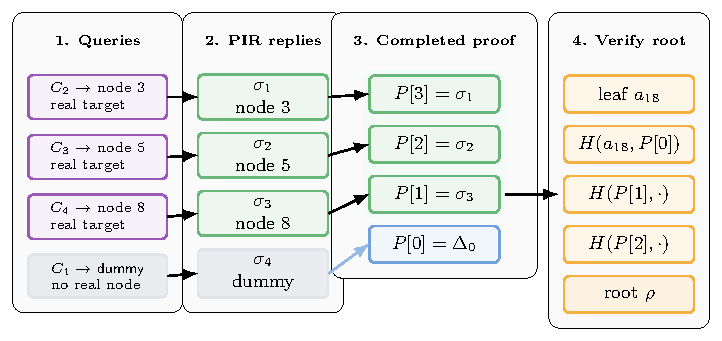
\includegraphics[width=\linewidth]{../figures/sparsetreepir_proof_completion_figure.pdf}
	\caption{One target-independent batch query and client-side proof reconstruction for leaf $18$.}
	\label{fig:completion}
\end{figure}

\begin{algorithm}[H]
\caption{Client-side proof reconstruction}
\label{alg:complete}
\begin{algorithmic}[1]
\Require Target leaf coordinate $\ell$, target leaf digest $a_0$, public metadata tables $\{\mathcal{M}_c\}_{c=1}^{m}$, client-side selection map $\{\tau_c\}_{c=1}^{m}$ from Algorithm~\ref{alg:query}, decoded PIR responses $\{\sigma_c\}_{c=1}^{m}$, default-empty hash chain $\{\Delta_t\}_{t=0}^{h-1}$
\Ensure Complete proof array $P[0..h-1]$ and reconstructed root digest $\rho$
\For{$t=0$ \textbf{to} $h-1$}
  \State Set $P[t]\gets \Delta_t$
\EndFor
\For{$c=1$ \textbf{to} $m$}
  \If{$\tau_c\neq\bot$}
    \State Read $(I_{\mathsf{srv}},\delta)\gets \mathcal{M}_c[\tau_c]$
    \State Set $P[\delta]\gets \sigma_c$
  \EndIf
\EndFor
\State $\rho\gets a_0$
\For{$t=0$ \textbf{to} $h-1$}
  \If{the $t$-th path bit of $\ell$ is $0$}
    \State $\rho\gets H(\rho\Vert P[t])$
  \Else
    \State $\rho\gets H(P[t]\Vert \rho)$
  \EndIf
\EndFor
\State \Return $P,\rho$
\end{algorithmic}
\end{algorithm}

\subsection{End-to-End Protocol Flow}

Putting these pieces together, the online flow for one target leaf is as follows. The client obtains its rank in the public ordered set of occupied leaves and performs one metadata lookup per color subdatabase. If the target rank lies in a stored target-rank interval, the client privately queries the corresponding record; otherwise, it sends a dummy PIR query to the same subdatabase. Thus every retrieval produces the same target-independent batch transcript: one well-formed PIR query per color. After decoding the PIR responses, the client uses its selection map to place the real non-default sibling digests into the proof array. All remaining positions are filled with public default hashes, and the client hashes upward along the target coordinate to obtain the SMT root.

\section{Correctness, Privacy, and Complexity}
\label{sec:correctness}

This section proves the correctness, privacy, and complexity properties of SparseTreePIR. The results are stated for the one-query-per-color retrieval model used by the construction: each retrievable proof node is stored in one color subdatabase, and each online retrieval sends one PIR query to every color subdatabase. For brevity in this section, we call the PIR-retrievable sibling nodes of Section~\ref{sec:model} \emph{active proof nodes}.

Let $N=|\mathcal{A}(T)|$ be the number of active proof nodes and let $n=|\mathcal{L}|$ be the number of occupied leaves. If $n=1$, then $\mathcal{A}(T)=\emptyset$, $m=0$, and no PIR query is needed. Unless otherwise stated, we assume $n\ge 2$.

\subsection{Width and Record Complexity}

The first result characterizes the number of colors needed by the one-query-per-color retrieval model.

\begin{theorem}[Tightness of $m$ in one-query-per-color retrieval]
\label{thm:mincolor}
Let
\[
m=\max_{\ell\in\mathcal{L}} |\mathsf{Path}(\ell)|.
\]
For a fixed height-$h$ SMT snapshot, $m$ colors are necessary and sufficient in the one-query-per-color retrieval model. A proper $m$-coloring can be computed in $O(N)$ time once the interval forest has been constructed. Moreover,
\[
m\le \min\{h,n-1\},
\]
and this bound is tight for every $h$ and $n\ge 2$.
\end{theorem}

\begin{proof}
For necessity, choose an occupied leaf $\ell^\star$ with $|\mathsf{Path}(\ell^\star)|=m$. All nodes in $\mathsf{Path}(\ell^\star)$ appear in the same membership proof. Therefore, any proper coloring must assign distinct colors to these $m$ nodes. Hence at least $m$ colors are necessary.

For sufficiency, consider the target-rank intervals $\{I_{\mathsf{srv}}(u):u\in\mathcal{A}(T)\}$. These intervals form a laminar family. Two active proof nodes can appear in the same membership proof exactly when their intervals contain the same target rank. In a laminar family, this is equivalent to one interval containing the other, i.e., to an ancestor-descendant relation in the corresponding interval forest. Thus, coloring each node by its depth in the interval forest is proper: two nodes at the same forest depth are not ancestor and descendant, so their intervals are disjoint and they cannot co-occur in one proof. The number of colors used by this depth coloring is the maximum number of target-rank intervals containing any target rank, which is exactly $m$. A single traversal of the interval forest computes this coloring in $O(N)$ time.

For the structural bound, every active proof node on a target path corresponds to a distinct SMT level whose sibling subtree is non-empty. Hence there are at most $h$ such nodes. In addition, the non-empty sibling subtrees on one target path are pairwise disjoint, and each contains at least one occupied leaf different from the target leaf. Therefore, the path contains at most $n-1$ active proof nodes. This proves $m\le \min\{h,n-1\}$.

The bound is tight. Let $k=\min\{h,n-1\}$ and choose the target leaf with logical bit string $0^h$. For each depth $d=0,\ldots,k-1$, add one occupied leaf in the sibling subtree that branches away from the target path at depth $d$, for example the bit string $0^d1\,0^{h-d-1}$. These $k$ leaves make $k$ different sibling subtrees on the target path non-empty, so the target proof contains $k$ active proof nodes. Any remaining occupied leaves can be added elsewhere without removing these witnesses. Hence the bound is attainable.
\end{proof}

\begin{remark}
Theorem~\ref{thm:mincolor} is where the SMT formulation departs most clearly from a naive complete-tree view. In a complete-tree layout, the batch profile is pinned to the full tree height $h$ regardless of how much non-default proof material exists. In the direct SMT formulation, the batch profile is governed instead by the maximum number of non-default sibling positions on any occupied-leaf proof. Consequently, the storage gain and the width gain are related but not identical: reducing the stored proof records is immediate, while reducing the number of color queries requires the proof-specific PIR record sets themselves to become smaller.
\end{remark}

\begin{lemma}[Number of active proof nodes]
\label{lem:activecount}
Let $n=|\mathcal{L}|$. Then
\[
|\mathcal{A}(T)| \le 2(n-1).
\]
The bound is tight for every binary occupied-leaf skeleton in which every branching internal node has two non-empty children represented in the SMT.
\end{lemma}

\begin{proof}
Every active proof node $u$ has a parent $p$ whose two original SMT children are both non-empty: $u$ is non-empty by definition, and $\operatorname{sib}(u)$ is also non-empty. Conversely, each branching parent with two non-empty children contributes at most its two child roots to $\mathcal{A}(T)$. Thus $|\mathcal{A}(T)|$ is at most twice the number of branching internal nodes in the compressed non-default skeleton induced by the occupied leaves.

Any finite rooted binary tree with $n$ leaves has at most $n-1$ branching internal nodes. Therefore $|\mathcal{A}(T)|\le 2(n-1)$. When the occupied-leaf skeleton is a full binary skeleton with $n-1$ branching internal nodes and both children of each branching node correspond to non-empty SMT subtrees, both child roots are active, giving equality.
\end{proof}

\subsection{Correctness}

We next prove that the coloring and retrieval procedures return exactly the non-default sibling digests needed for a standard SMT membership proof.

\begin{proposition}[Validity of subtree color permutations]
\label{prop:permvalid}
Let $\varphi$ be a proper coloring, let $U$ be any rooted subtree of the interval forest, and let $A(U)\subseteq[m]$ be the set of colors not used on the strict ancestor chain of $U$. Assume every node in $U$ is colored from $A(U)$. If $\pi$ is any permutation of $A(U)$, and every node $x\in U$ is recolored from $\varphi(x)$ to $\pi(\varphi(x))$ while all nodes outside $U$ keep their colors, then the resulting coloring is still proper.
\end{proposition}

\begin{proof}
Consider any two nodes that may appear together in one proof. If both lie outside $U$, nothing changes. If both lie inside $U$, they were originally assigned distinct colors under $\varphi$, and applying the same permutation $\pi$ preserves distinctness because $\pi$ is injective on $A(U)$. It remains to consider a pair consisting of one node $x\in U$ and one node $y\notin U$.

If $x$ and $y$ can co-occur on a proof path, then $y$ must be an ancestor of the subtree root of $U$, because nodes outside $U$ but incomparable with $U$ correspond to disjoint intervals and cannot appear on the same path. By definition, every ancestor color is excluded from $A(U)$. Therefore $\pi(\varphi(x))\in A(U)$ can never equal $\varphi(y)$, and the pair remains properly colored. Hence no violating ancestor-descendant pair is created, so the recolored assignment is valid.
\end{proof}

\begin{proposition}[Per-color uniqueness on proof paths]
\label{prop:unique}
If $\varphi$ is a proper coloring, then for every occupied leaf $\ell\in\mathcal{L}$ and every color $c\in[m]$, the set $\mathsf{Path}(\ell)$ contains at most one active proof node of color $c$.
\end{proposition}

\begin{proof}
If there were two distinct nodes $u,v\in\mathsf{Path}(\ell)$ with $\varphi(u)=\varphi(v)=c$, the definition of proper coloring would be violated.
\end{proof}

\begin{proposition}[Fixed-size batch retrieval]
\label{prop:batch}
Assume a correct single-item PIR backend. Then any proper coloring lets the client recover all active proof nodes of a target leaf $\ell$ using one batch-PIR request with exactly $m$ PIR subqueries.
\end{proposition}

\begin{proof}
By Proposition~\ref{prop:unique}, each color subdatabase contains at most one node from $\mathsf{Path}(\ell)$. Therefore, for each color, the client either sends a PIR query for the unique real record in that subdatabase, or sends a dummy PIR query when no such record exists. Correctness of the PIR scheme returns the selected digest in every real color. These returned digests are exactly the non-default sibling digests in $\mathsf{Path}(\ell)$.
\end{proof}

\begin{proposition}[Correctness of default-hash completion]
\label{prop:complete}
Assume that the underlying single-item PIR scheme is correct. If $\varphi$ is a proper coloring, then Algorithm~\ref{alg:complete} reconstructs the complete SMT proof of the target leaf $\ell$ from the real PIR outputs and the public default-empty hash chain.
\end{proposition}

\begin{proof}
Fix a proof level $t\in\{0,\ldots,h-1\}$. If the sibling subtree at level $t$ is non-empty, then its digest is an active proof node. This node belongs to $\mathsf{Path}(\ell)$, appears in exactly one color subdatabase by Proposition~\ref{prop:unique}, and is retrieved correctly by Algorithm~\ref{alg:query}. Algorithm~\ref{alg:complete} writes this digest into the proof slot $P[t]$. If the sibling subtree at level $t$ is empty, then its digest is the public default value $\Delta_t$, and Algorithm~\ref{alg:complete} leaves $P[t]=\Delta_t$. Hence every proof slot contains the correct sibling digest. The client can therefore recompute the SMT root by the standard bottom-up Merkle verification procedure.
\end{proof}

\subsection{Target Privacy}

We now prove target privacy relative to the setup leakage defined in Section~\ref{sec:model}.

\begin{theorem}[Target privacy under setup leakage]
\label{prop:privacy}
Assume the setup leakage profile and the target-privacy game in Definition~\ref{def:privacygame}. Assume also that the retrieval width $m$ is polynomially bounded in the security parameter, as holds when the SMT height $h$ is polynomially bounded because $m\le h$. If each underlying single-item PIR query is query-private over its corresponding color subdatabase, and if dummy queries are sampled from a distribution computationally indistinguishable from well-formed PIR queries over that same subdatabase, then the batch retrieval protocol is target-private relative to $\mathcal{L}_{\mathsf{setup}}(T)$.
\end{theorem}

\begin{proof}
Fix any efficient adversary and any two occupied target leaves $\ell_0,\ell_1$ chosen in the game. Condition on the setup leakage $\mathcal{L}_{\mathsf{setup}}(T)$. The adversary already knows the SMT snapshot information included in the leakage, the active proof nodes, the coloring, the public metadata tables, the color subdatabase sizes, and the fact that every retrieval sends one PIR query to each color subdatabase. Therefore, the only target-dependent part of the online transcript is the sequence of PIR queries.

Consider one color $c$. For target $\ell_b$, Algorithm~\ref{alg:query} either queries the unique real index in $\mathcal{D}_c$ whose target-rank interval contains the target rank, or sends a dummy query over the same subdatabase. If both targets induce real queries, single-item PIR query privacy makes the two selected indices computationally indistinguishable. If one target induces a real query and the other induces a dummy query, the dummy query is still distributed as a well-formed PIR query over the same subdatabase, and PIR query privacy hides whether the selected index is meaningful. If both targets induce dummy queries, the two query distributions are identical up to target-independent randomness.

A standard hybrid argument over the $m$ colors shows that the complete batch transcript for $\ell_0$ is computationally indistinguishable from the complete batch transcript for $\ell_1$. Since $m$ is polynomially bounded, the hybrid loss is negligible. Thus every efficient adversary has negligible advantage in the target-privacy game.
\end{proof}

\subsection{Load Balance}

Correctness and privacy require only a proper coloring. The running time of a PIR backend, however, depends on the sizes of the color subdatabases. We therefore analyze the maximum subdatabase size.

\begin{lemma}[Same-color intervals are disjoint]
If $\varphi$ is a proper coloring, then for any color $c$, any two distinct intervals in
\[
\mathcal{I}_c=\{I_{\mathsf{srv}}(u): \varphi(u)=c\}
\]
are disjoint.
\end{lemma}

\begin{proof}
Suppose two distinct same-color nodes $u$ and $v$ had overlapping target-rank intervals. Then some occupied-leaf rank would be contained in both intervals, so the corresponding membership proof would contain both $u$ and $v$. This contradicts Proposition~\ref{prop:unique}.
\end{proof}

\begin{theorem}[Structural lower bound for color-subdatabase balance]
\label{thm:structlb}
Let $N=|\mathcal{A}(T)|$ and let $m$ be the number of colors. For a node $v$ in the interval forest, let $d(v)$ be the number of active proof nodes on the path from the root of its connected component to $v$, including $v$, and let $\operatorname{desc}(v)$ be the number of strict descendants of $v$. Define
\[
B(T)=
\max\left\{
\left\lceil \frac{N}{m}\right\rceil,\,
\max_{v:\ d(v)<m}
\left\lceil \frac{\operatorname{desc}(v)}{m-d(v)}\right\rceil
\right\}.
\]
If the second maximum is over an empty set, it is omitted.
Then every proper coloring $\varphi:\mathcal{A}(T)\rightarrow[m]$ satisfies
\[
\max_{c\in[m]} |\mathcal{D}_c| \ge B(T).
\]
\end{theorem}

\begin{proof}
The term $\lceil N/m\rceil$ is the equal-split lower bound. For the second term, fix a node $v$ with $d(v)<m$. The $d(v)$ nodes on the path from the component root to $v$ must have distinct colors. Every strict descendant of $v$ co-occurs with each of these path nodes in some proof and therefore cannot use any of their $d(v)$ colors. Hence the $\operatorname{desc}(v)$ strict descendants must be assigned to at most $m-d(v)$ remaining colors. By the pigeonhole principle, at least one color subdatabase contains at least
\[
\left\lceil \frac{\operatorname{desc}(v)}{m-d(v)}\right\rceil
\]
of these descendants. Taking the maximum over all such $v$ and combining it with the equal-split bound proves the claim.
\end{proof}

\begin{proposition}[A posteriori balance certificate and termination]
\label{prop:activebalancecert}
Let $\varphi_{\mathsf{out}}$ be the coloring returned by Algorithm~\ref{alg:activebalance}, and let
\[
U=\max_{c\in[m]}|\mathcal{D}_c(\varphi_{\mathsf{out}})|.
\]
Let $\operatorname{OPT}$ be the smallest possible value of $\max_c|\mathcal{D}_c|$ over all proper $m$-colorings. Then
\[
\frac{U}{\operatorname{OPT}}\le \frac{U}{B(T)}.
\]
Thus $U/B(T)$ is an a posteriori balance certificate for the returned coloring. Moreover, Algorithm~\ref{alg:activebalance} accepts only finitely many improving moves. If it stops because no candidate subtree permutation improves the load vector, then the returned coloring is a local optimum under the allowed subtree-permutation moves.
\end{proposition}

\begin{proof}
By Theorem~\ref{thm:structlb}, $\operatorname{OPT}\ge B(T)$. Therefore
\[
\frac{U}{\operatorname{OPT}}\le \frac{U}{B(T)}.
\]
This proves the certificate.

For termination, every accepted move strictly decreases the lexicographically sorted load vector $\Psi(\varphi)=\mathrm{sort}_{\downarrow}(|\mathcal{D}_1|,\ldots,|\mathcal{D}_m|)$. There are finitely many colorings of the finite interval forest over the fixed color set $[m]$. Therefore, the algorithm cannot accept infinitely many strictly improving moves. If a pass finds no improving candidate, then no subtree permutation considered by the algorithm can further decrease $\Psi$, which is exactly local optimality with respect to this move set.
\end{proof}

\subsection{Indexing and Runtime Complexity}

The remaining results give the preprocessing, balancing, and online client costs.

\begin{theorem}[Indexing complexity]
\label{thm:index}
Let $N=|\mathcal{A}(T)|$ be the total number of active proof nodes, and let $N_c=|\mathcal{D}_c|$ be the size of color subdatabase $c$. Then the interval metadata construction and query indexing satisfy
\begin{align*}
&\text{preprocessing time} \in O(N\log N),\\
&\text{preprocessing space} \in O(N),\\
&\text{single-retrieval indexing time} \in O(m\log N).
\end{align*}
\end{theorem}

\begin{proof}
Computing the target-rank interval and proof level for each active proof node takes $O(N)$ time once the compressed non-default skeleton is available. Sorting the metadata tables costs
\[
O\!\left(\sum_{c=1}^{m}N_c\log N_c\right)\subseteq O(N\log N).
\]
At query time, the client performs one binary search per color, which costs
\[
O\!\left(\sum_{c=1}^{m}\log N_c\right)\subseteq O(m\log N).
\]
The active digest records and their interval metadata require $O(N)$ space.
\end{proof}

\begin{theorem}[ActiveBalance complexity]
\label{thm:activebalancecomplexity}
Given a proper coloring of an interval forest with $N$ active proof nodes and $m$ colors, one execution of Algorithm~\ref{alg:activebalance} with at most $R_1$ passes runs in
\[
O(R_1 N m^3)
\]
time and uses $O(Nm)$ additional space.
\end{theorem}

\begin{proof}
In one pass, Algorithm~\ref{alg:activebalance} computes, for each subtree root, the colors used by its ancestors and the per-color counts inside the subtree. These histograms require $O(Nm)$ space and can be computed in $O(Nm)$ time by a bottom-up traversal.

For a fixed subtree root $U$, the available-color set has size at most $m$. Building the local cost matrix $K_U$ takes $O(m^2)$ time, and solving the resulting assignment problem using the Hungarian algorithm takes $O(m^3)$ time. Checking the induced global load vector costs $O(m)$, which is dominated by $O(m^3)$. Evaluating all $N$ subtree roots therefore costs $O(Nm^3)$ per pass and $O(R_1Nm^3)$ over $R_1$ passes.

The peak additional storage is $O(Nm)$.
\end{proof}

\begin{theorem}[Client-side completion complexity]
\label{thm:complete}
Assume that the public metadata tables $\{\mathcal{M}_c\}_{c=1}^{m}$ are already available and that the default-empty hash chain $\Delta_0,\ldots,\Delta_{h-1}$ has been precomputed once. Then Algorithm~\ref{alg:complete} runs in $O(h)$ time and uses $O(h)$ additional space. Consequently, the total online client work for query indexing and proof completion is
\[
O(m\log N + h).
\]
\end{theorem}

\begin{proof}
Algorithm~\ref{alg:complete} initializes a proof array of length $h$, processes at most one real PIR output per color, and performs exactly $h$ bottom-up hash computations. Thus its time and space costs are both $O(h)$. Combining this with the $O(m\log N)$ indexing cost from Theorem~\ref{thm:index} gives the stated bound. The default-empty hash chain is public and can be precomputed once in $O(h)$ time and space.
\end{proof}

The following theorem states the end-to-end guarantee used in the evaluation: it ties the construction to correctness, target privacy, storage, metadata, and PIR workload cost.

\begin{theorem}[End-to-end SparseTreePIR guarantee]
\label{thm:endtoend}
Fix a public height-$h$ SMT snapshot $T$ with active proof-node set $\mathcal{A}(T)$, number of colors $m$, a proper coloring $\varphi$, color subdatabases $\mathcal{D}_1,\ldots,\mathcal{D}_m$, and public metadata tables $\mathcal{M}_1,\ldots,\mathcal{M}_m$. Assume that the underlying single-item PIR backend is correct and query-private for each subdatabase, and that dummy queries are sampled from the same query distribution as well-formed PIR queries over the corresponding subdatabase. Then SparseTreePIR satisfies the following end-to-end guarantee for every occupied target leaf:
\begin{enumerate}[leftmargin=2em]
  \item the client reconstructs a valid standard height-$h$ SMT membership proof;
  \item the retrieval is target-private relative to the setup leakage in Definition~\ref{def:leakagefunction} and the target-privacy game in Definition~\ref{def:privacygame};
  \item the PIR database contains exactly $N=|\mathcal{A}(T)|$ digest records, and the public metadata size is $O(N)$;
  \item client-side lookup and proof completion together cost $O(m\log N+h)$ time;
  \item the PIR-backend workload is determined by the load vector $(|\mathcal{D}_1|,\ldots,|\mathcal{D}_m|)$: a sequential execution performs one PIR query over each color subdatabase, while a parallel execution is bottlenecked by the largest per-color backend call.
\end{enumerate}
\end{theorem}

\begin{proof}
The first item follows from Proposition~\ref{prop:batch} and Proposition~\ref{prop:complete}: the client privately retrieves all non-default sibling digests and fills the remaining proof slots with public default hashes. The second item follows from Theorem~\ref{prop:privacy}. For the third item, the construction stores one digest for every active proof node, and each metadata entry contains a constant number of fields. The fourth item combines Theorem~\ref{thm:index} and Theorem~\ref{thm:complete}. Finally, Algorithm~\ref{alg:query} issues one independent PIR query to each color subdatabase, so the backend workload composes over the color subdatabase sizes. Under parallel execution, the largest per-color backend call determines the bottleneck.
\end{proof}

\begin{remark}
Algorithms~\ref{alg:query} and~\ref{alg:complete} are directly implementable: all inputs required by proof completion are either public metadata, public default hashes, or client-local state already produced during query generation. No additional server round is needed after batch-PIR extraction.
\end{remark}


\section{Experimental Evaluation}
\label{sec:experiments}

This section evaluates SparseTreePIR as a PIR-based retrieval layout for membership proofs in fixed public SMT snapshots. Direct SMT proof serving is used only as a functional reference, not as a privacy-preserving baseline, because a direct request reveals the queried coordinate and authentication path. We therefore compare SparseTreePIR with alternative privacy-preserving layouts that expose different database sizes, query patterns, and subdatabase sizes to the same PIR backends. The evaluation asks four questions: (i) what database and query profile is induced by real SMT key sets; (ii) how much improvement comes from storing only non-default proof records; (iii) how much does \ActiveBalance{} reduce the maximum per-color subdatabase size; and (iv) whether these layout-level improvements translate into lower communication and runtime with existing PIR backends.

\subsection{Workloads, Platform, and Metrics}

We use six SMT key sets. Five are address-derived account-key workloads from public Polygon zkEVM and ZKsync Era RPC data, and one is a FuelLabs SMT test-vector workload. The Polygon workloads expand observed addresses into the Polygon SMT key types for balance, nonce, code hash, and code-hash length. The recent Polygon workload covers blocks $32{,}046{,}547$--$32{,}096{,}546$; the multi-window and broad variants sample four and eleven historical windows, respectively. The ZKsync sample and broad workloads cover blocks $70{,}082{,}262$--$70{,}132{,}261$ and $69{,}632{,}271$--$70{,}132{,}270$, expanding addresses into balance, nonce, code, and storage-root keys. The FuelLabs workload is generated from the \texttt{smt\_test\_spec.json} fixture in \texttt{FuelLabs/smt-test-generation}. These workloads are not full deployed state-tree dumps; they are reproducible account-key snapshots intended to stress the retrieval layouts induced by realistic account-key distributions rather than to reproduce a complete archival state service. Exact source files, extraction scripts, block windows, and summary metadata are included in the artifact.

Each key set is mapped into height-$128$ and height-$256$ SMT coordinate spaces. Polygon and ZKsync keys are first hashed with SHA-256 and then mapped by prefix; FuelLabs vectors use their hexadecimal prefix coordinates. Duplicate input keys and duplicate coordinates after mapping are merged into one occupied SMT leaf. The main workload suite contains no synthetic random-leaf trees.

Structural metrics are deterministic functions of the mapped key set and the interval representation of PIR records: the number of PIR records $N=|\mathcal{A}(T)|$, the number of subqueries $m$, the maximum per-color subdatabase size $M(\varphi)=\max_c|\mathcal{D}_c|$, the dummy-query fraction, and the public metadata size. These quantities characterize the workload exposed to the PIR backend. A backend whose cost depends on database size is driven by the subdatabase-size vector $(|\mathcal{D}_1|,\ldots,|\mathcal{D}_m|)$: sequential work composes across queried subdatabases, while parallel work is typically limited by the largest backend call.

Implementation-based backend measurements were run on Ubuntu 22.04.5 with Linux 6.8, a 13th Gen Intel Core i5-13500HX CPU with 20 hardware threads, 15 GiB RAM, Python 3.10.12, Go 1.18.1, GCC/G++ 11.4, and CMake 3.22. The SimplePIR and PIANO checkouts are pinned at commits \texttt{e9020b03bf28} and \texttt{f7107cfadc15}, respectively; the artifact records the full hashes, environment, command lines, and seed-level CSVs. The machine does not expose AVX-512, so YPIR is not treated as an evaluated backend.

For backend experiments, we use the height-$128$ workloads and compare the PBC-style SMT baseline against SparseTreePIR. Each backend experiment is repeated with three target-sampling seeds, $73000$, $83000$, and $93000$, and each seed requests $50$ occupied targets per workload. Communication is deterministic once the layout and backend parameter tier are fixed, so its standard deviation is zero across repeated runs; timing columns report the sample standard deviation over target-sampling seeds. Online communication counts backend upload and download bytes for the measured PIR calls. Setup time refers only to backend preprocessing for the measured databases, while query time refers to client query generation. Server response generation, client-side proof reconstruction, one-time layout construction, and public metadata publication are excluded from those timing columns unless reported separately.

\subsection{Privacy-Preserving Layouts}

We compare five privacy-preserving retrieval layouts. \emph{Complete-tree TreePIR} treats the SMT as a complete height-$h$ perfect tree and is used only as an accounting baseline, because a height-$128$ or height-$256$ full coordinate tree is not materializable. \emph{Height-preserving pruned TreePIR} removes public default records from the searched payloads but keeps a height-$h$ query pattern. \emph{PBC-style SMT} is an optimistic generic batch-placement baseline over the same active proof records: it stores three replicated copies and spreads them over $\lceil1.5m\rceil$ buckets. Our implementation uses deterministic balanced placement rather than sampled Cuckoo placement when reporting bucket sizes, giving this baseline optimistic load balance and removing seed dependence. \emph{Unpartitioned active-record PIR} stores active proof records once but searches one global active-record database for each proof slot. \emph{SparseTreePIR} stores the same active proof records once, partitions them into per-color subdatabases, and applies \ActiveBalance{} to reduce the maximum subdatabase size.

\paragraph{Height-preserving pruned TreePIR baseline.}
For each verifier proof slot $i\in[h]$, let $\mathcal{P}_i$ be the set of non-default sibling digests that can appear in slot $i$ across occupied-leaf membership proofs. This baseline searches only these non-default records, but online retrieval still sends one query for every proof level, using a dummy query when the target proof has no non-default sibling at that level. Its query width is therefore $h$, and its maximum subdatabase size is $\max_i|\mathcal{P}_i|$. This baseline tests whether simply deleting default records is sufficient once the protocol has already committed to a height-$h$ query pattern.

\begin{table*}[!t]
\centering
\caption{SMT workload profiles and induced costs for privacy-preserving retrieval layouts.}
\label{tab:real_workload_shape}
\scriptsize
\setlength{\tabcolsep}{4pt}
\begin{tabular}{lrrrrrrrrrr}
\toprule
Workload & $h$ & Keys & PIR rec. & Subq. $m$ & Avg. rec. & Dummy & Pruned q/max & PBC b/max & Unpart. max & STPIR max \\
\midrule
FuelLabs SMT vectors & 128 & 100   & 198   & 9  & 6.88 & 23.56\% & 128 / 40  & 14 / 43   & 198   & 23 \\
FuelLabs SMT vectors & 256 & 100   & 198   & 9  & 6.88 & 23.56\% & 256 / 40  & 14 / 43   & 198   & 23 \\
Polygon recent       & 128 & 384   & 766   & 11 & 8.89 & 19.15\% & 128 / 168 & 17 / 136  & 766   & 70 \\
Polygon recent       & 256 & 384   & 766   & 11 & 8.89 & 19.15\% & 256 / 168 & 17 / 136  & 766   & 70 \\
ZKsync sample        & 128 & 956   & 1910  & 13 & 10.19 & 21.62\% & 128 / 370 & 20 / 287  & 1910  & 147 \\
ZKsync sample        & 256 & 956   & 1910  & 13 & 10.19 & 21.62\% & 256 / 370 & 20 / 287  & 1910  & 147 \\
Polygon multi-window & 128 & 1348  & 2694  & 14 & 10.73 & 23.36\% & 128 / 530 & 21 / 385  & 2694  & 193 \\
Polygon multi-window & 256 & 1348  & 2694  & 14 & 10.73 & 23.36\% & 256 / 530 & 21 / 385  & 2694  & 193 \\
Polygon broad        & 128 & 7040  & 14078 & 17 & 13.11 & 22.86\% & 128 / 2762 & 26 / 1625 & 14078 & 829 \\
Polygon broad        & 256 & 7040  & 14078 & 17 & 13.11 & 22.86\% & 256 / 2762 & 26 / 1625 & 14078 & 829 \\
ZKsync broad         & 128 & 7740  & 15478 & 17 & 13.25 & 22.03\% & 128 / 3014 & 26 / 1786 & 15478 & 911 \\
ZKsync broad         & 256 & 7740  & 15478 & 17 & 13.25 & 22.03\% & 256 / 3014 & 26 / 1786 & 15478 & 911 \\
\bottomrule
\end{tabular}
\end{table*}

In Table~\ref{tab:real_workload_shape}, PIR rec. is the number of PIR records, Subq. $m$ is the number of SparseTreePIR subqueries, Dummy is the fraction of dummy queries, Pruned q/max reports the query count and maximum subdatabase size of the height-preserving pruned TreePIR baseline, PBC b/max reports $\lceil1.5m\rceil$ buckets and the largest PBC bucket, and STPIR max is the largest SparseTreePIR subdatabase after \ActiveBalance{}. The table shows that the PIR database can be much smaller than the logical SMT proof space while preserving the standard height-$h$ verification interface. Across the workload suite, SparseTreePIR uses only $9$--$17$ subqueries, whereas the pruned TreePIR baseline still issues $128$ or $256$ queries. For the broad ZKsync workload, for example, $15478$ active proof records are partitioned into $17$ subdatabases, and the largest subdatabase contains $911$ records; the Pruned TreePIR-$128$ baseline has a largest subdatabase of $3014$ records. Increasing the logical height from $128$ to $256$ does not change these active records for the measured key sets because the occupied-leaf skeleton has already separated; the client reconstructs the remaining proof levels using public default hashes.

\begin{table}[!t]
\centering
\caption{Measured sources of improvement on the real SMT workload suite. Multiplicative gains are computed from arithmetic-mean reductions over the six height-$128$ workload instances.}
\label{tab:real_gain_sources}
\scriptsize
\setlength{\tabcolsep}{3pt}
\resizebox{\linewidth}{!}{%
\begin{tabular}{p{0.30\linewidth}p{0.30\linewidth}p{0.32\linewidth}}
\toprule
Comparison & Observed resource effect & Interpretation \\
\midrule
vs. complete-tree TreePIR & Full $h=128/256$ layouts are $>4.3{\cdot}10^{34}\times$ / $>10^{73}\times$ larger than the largest active-record layout & Full coordinate trees are mismatched to sparse SMT proof retrieval. \\
vs. pruned TreePIR & $9.5\times$ fewer subqueries; $2.5\times$ smaller maximum subdatabase & Deleting default records still leaves a height-$h$ query pattern. \\
vs. PBC-style SMT & $1.5\times$ fewer subqueries; $1.9\times$ smaller largest bucket & Generic batch placement ignores authentication-path structure. \\
vs. unpartitioned active-record PIR & $12.7\times$ smaller maximum searched database & Storing only non-default records is insufficient without partitioning. \\
vs. node-local coloring & $1.2\times$ smaller maximum subdatabase & \ActiveBalance{} improves a valid coloring without changing $m$. \\
\bottomrule
\end{tabular}
\par}
\end{table}

Table~\ref{tab:real_gain_sources} separates the source of each improvement. Complete-tree TreePIR uses a layout that is natural for dense Merkle trees but inflated for sparse SMT snapshots. The height-preserving pruned baseline removes default records but still keeps a height-$h$ query pattern. PBC-style SMT uses the active proof records but treats them as an arbitrary batch, paying for replication and extra buckets. The unpartitioned active-record baseline stores only non-default proof records but repeatedly searches one large database. SparseTreePIR combines non-default proof-record storage, a reduced query count $m$, and balanced per-color subdatabases.

Overall, the evaluation isolates three effects. Storing only non-default proof records removes the full coordinate tree from the PIR database, avoiding a complete-tree layout that is more than $10^{34}\times$ larger even at height $128$. SparseTreePIR then replaces the height-$h$ pruned TreePIR query pattern with $m$ subqueries, giving $9.5\times$ fewer subqueries and a $2.5\times$ smaller maximum subdatabase on the height-$128$ workloads. It also gives $1.5\times$ fewer subqueries than the PBC-style baseline and a $12.7\times$ smaller searched database than unpartitioned active-record PIR. \ActiveBalance{} reduces the largest subdatabase by another $1.2\times$ without changing $m$. These effects are orthogonal to the choice of PIR backend; the implementation-based experiments below measure whether the improved layout profile carries over to existing PIR systems.

\subsection{Effect of \ActiveBalance{}}

A valid coloring is not automatically a good backend layout. Table~\ref{tab:real_activebalance} compares \ActiveBalance{} with a node-local greedy initializer on the height-$128$ workloads. The initializer assigns feasible colors using ancestor-color constraints and current global loads, but it does not apply subtree-level color permutations. Both schemes use the same active proof records and the same number of colors; the only difference is the balancing refinement. The Lower column is the structural lower bound $B(T)$ from Theorem~\ref{thm:structlb}.

\begin{table}[!t]
\centering
\caption{\ActiveBalance{} ablation on real height-$128$ workloads}
\label{tab:real_activebalance}
\scriptsize
\setlength{\tabcolsep}{3pt}
\resizebox{\linewidth}{!}{%
\begin{tabular}{lrrrrrrr}
\toprule
Workload & PIR rec. & $m$ & Lower & Greedy max & AB max & Red. & Meta KB \\
\midrule
FuelLabs SMT vectors & 198   & 9  & 22  & 26   & 23  & 11.5\% & 4.6 \\
Polygon recent       & 766   & 11 & 70  & 83   & 70  & 15.7\% & 18.0 \\
ZKsync sample        & 1910  & 13 & 147 & 180  & 147 & 18.3\% & 44.8 \\
Polygon multi-window & 2694  & 14 & 193 & 236  & 193 & 18.2\% & 63.1 \\
Polygon broad        & 14078 & 17 & 829 & 929  & 829 & 10.8\% & 330.0 \\
ZKsync broad         & 15478 & 17 & 911 & 1162 & 911 & 21.6\% & 362.8 \\
\bottomrule
\end{tabular}
\par}
\end{table}

In five of the six height-$128$ workloads, \ActiveBalance{} reaches the reported structural lower bound exactly; in the Fuel test-vector workload it is within $1.045\times$ of the lower bound. The reduction in maximum subdatabase size ranges from $10.8\%$ to $21.6\%$ relative to the greedy initializer. The metadata column uses the prototype encoding of $24$ public bytes per active proof record, compared with $32$ private digest bytes per record. Thus the public lookup state is linear in the number of active proof records and remains independent of the full logical coordinate space.

\subsection{Experiments with Existing PIR Backends}

We next evaluate whether the structural improvements translate to existing PIR implementations. The SimplePIR integration materializes the $32$-byte digest records for each subdatabase and calls the official SimplePIR Go API~\cite{simplepir}, including \texttt{Setup}, \texttt{Query}, \texttt{Answer}, and \texttt{Recover}. Each digest is retrieved as eight $32$-bit chunks because the artifact's database constructor represents one entry as a machine word. The bridge verifies recovered chunks, so this is an end-to-end digest-retrieval experiment, although it is not optimized for digest packing.

The PIANO integration uses the public PIANO artifact~\cite{piano} with the subdatabase-size vector induced by each workload layout. It evaluates backend behavior under the layout-induced database sizes, but it does not implement full SMT proof reconstruction. PIANO's artifact internally caps the number of subdatabase queries according to its refresh window for small databases; the raw tables record the completed subdatabase-level query counts. We therefore treat PIANO as a secondary implementation-based check, while SimplePIR is the primary end-to-end backend experiment.

\begin{table}[!t]
\centering
\caption{Repeated implementation-based backend results on real height-$128$ workloads. Each entry is a baseline/SparseTreePIR cost ratio averaged over six workloads, three seeds, and $50$ requested occupied targets per seed. Server-response gain is SimplePIR response-generation time; preprocessing gain is backend preprocessing only and excludes layout construction and metadata publication.}
\label{tab:real_backend_summary}
\scriptsize
\setlength{\tabcolsep}{3pt}
\resizebox{\linewidth}{!}{%
\begin{tabular}{lrrrrrrr}
\toprule
Backend & Runs & Query-count gain & Max-size gain & Comm. gain & Client-query gain & Server-response gain & Preproc. gain \\
\midrule
SimplePIR full API & $3\times50$ & $1.5\times$ & -- & $2.1\times$ & $1.7\times$ & $1.8\times$ & $2.3\times$ \\
PIANO local runner & $3\times50$ & $1.5\times$ & $1.9\times$ & $2.3\times$ & $2.4\times$ & -- & $3.1\times$ \\
\bottomrule
\end{tabular}
\par}
\end{table}

Table~\ref{tab:real_backend_summary} is the main backend result. Against the PBC-style SMT baseline, SparseTreePIR gives $2.1\times$ lower online communication under SimplePIR and $2.3\times$ lower online communication under PIANO. Under SimplePIR, server response-generation time is $1.8\times$ lower on average. PIANO answer-time measurements are not reported because the artifact's small-database counters are often zero or quantized. Client query generation and backend preprocessing also improve, with gains ranging from $1.7\times$ to $3.1\times$. These gains are not caused by changing the PIR primitive: both schemes are measured through the same backend in each row. They come from the database layout exposed to the backend: the PBC-style baseline stores three copies over approximately $1.5m$ buckets, whereas SparseTreePIR stores one copy over $m$ subdatabases.

\begin{table}[!t]
\centering
\caption{Raw SimplePIR full-API means behind Table~\ref{tab:real_backend_summary}. Values are arithmetic means over the three target-sampling seeds; communication is KB per requested proof and timings are milliseconds.}
\label{tab:simplepir_raw_means}
\scriptsize
\setlength{\tabcolsep}{3pt}
\resizebox{\linewidth}{!}{%
\begin{tabular}{lrrrrrr}
\toprule
Workload & PBC KB & Sparse KB & PBC query & Sparse query & PBC answer & Sparse answer \\
\midrule
Fuel vectors        & 12.000 & 5.906  & 9.061  & 5.936  & 0.033 & 0.023 \\
Polygon recent      & 25.500 & 11.688 & 12.180 & 7.609  & 0.044 & 0.029 \\
ZKsync sample       & 43.125 & 20.719 & 15.817 & 9.684  & 0.076 & 0.038 \\
Polygon multi-window& 51.844 & 25.375 & 17.792 & 10.633 & 0.081 & 0.047 \\
Polygon broad       & 133.250& 62.156 & 32.367 & 17.223 & 0.245 & 0.114 \\
ZKsync broad        & 138.938& 65.344 & 32.302 & 17.679 & 0.268 & 0.120 \\
\bottomrule
\end{tabular}
\par}
\end{table}

Table~\ref{tab:simplepir_raw_means} gives the absolute SimplePIR values behind the aggregate ratios. The ratios in Table~\ref{tab:real_backend_summary} are computed from per-workload reductions, so they need not equal ratios of rounded arithmetic means in the raw table. The artifact also includes an aggregate raw-means CSV for both SimplePIR and PIANO, including backend setup time.

\begin{table}[!t]
\centering
\caption{Per-workload implementation-based backend gains against the PBC-style SMT baseline. Query count reports PBC-style buckets / SparseTreePIR colors; other entries are baseline/SparseTreePIR cost ratios averaged over three seeds.}
\label{tab:real_backend_workloads}
\scriptsize
\setlength{\tabcolsep}{3pt}
\resizebox{\linewidth}{!}{%
\begin{tabular}{lrrrrrr}
\toprule
Workload & Query count & SimplePIR comm. & SimplePIR query & PIANO comm. & PIANO query & PIANO max size \\
\midrule
FuelLabs SMT vectors & 14 / 9  & $2.0\times$ & $1.5\times$ & $3.2\times$ & $3.4\times$ & $1.9\times$ \\
Polygon recent       & 17 / 11 & $2.2\times$ & $1.6\times$ & $3.1\times$ & $2.7\times$ & $1.9\times$ \\
ZKsync sample        & 20 / 13 & $2.1\times$ & $1.6\times$ & $2.1\times$ & $1.8\times$ & $2.0\times$ \\
Polygon multi-window & 21 / 14 & $2.0\times$ & $1.7\times$ & $2.1\times$ & $2.1\times$ & $2.0\times$ \\
Polygon broad        & 26 / 17 & $2.1\times$ & $1.9\times$ & $2.1\times$ & $3.1\times$ & $2.0\times$ \\
ZKsync broad         & 26 / 17 & $2.1\times$ & $1.8\times$ & $2.1\times$ & $2.1\times$ & $2.0\times$ \\
\bottomrule
\end{tabular}
\par}
\end{table}

Table~\ref{tab:real_backend_workloads} shows that the communication reduction is stable across workloads. SimplePIR online communication is $2.0\times$--$2.2\times$ lower, and PIANO online communication is $2.1\times$--$3.2\times$ lower. Timing gains vary more than communication because they depend on backend parameter tiers, refresh behavior, and small-database effects; the SimplePIR answer-time values are especially small and should be read as supporting evidence rather than as the primary performance metric. The more stable evidence is the deterministic communication reduction and the improved database profile, both of which hold across all repeated measurements.

\subsection{Reproducibility and Scope}

All tables in this section are generated from repository scripts and checked-in CSV outputs. The repeated backend run writes per-seed raw tables, per-seed summaries, aggregate mean and standard-deviation tables, and an environment record. The structural tables are deterministic for the input key sets; backend timing tables are repeated because implementation timings are machine-dependent. Communication is reported as backend upload and download bytes for the measured PIR calls and does not include one-time publication of public metadata.

The scope of the evidence is intentionally limited. The SimplePIR bridge and PIANO experiment are the concrete backend integrations used for the main claims. The local LWE-style prototype, two-server XOR model, and public TreePIR artifact smoke tests are useful for development and appendix-level context, but they are not used as primary backend evidence in this section. In particular, the TreePIR VBPIR and Spiral artifacts operate on full-tree TreePIR layouts; a full SparseTreePIR integration would require exporting the per-color subdatabases into each backend-specific database encoding and validating the corresponding extraction procedure. YPIR is not evaluated on this platform because the machine lacks AVX-512 support, and a SealPIR-style service integration requires a heavier SEAL, Protobuf, and gRPC build stack. These systems are future integration targets rather than unreported completed experiments.

The protocol scope is also fixed. We evaluate membership-proof retrieval for occupied leaves in a fixed public SMT snapshot. Non-membership retrieval over absent coordinates would require a different interval domain, a different leakage model, and explicit treatment of whether the present-versus-absent query type is hidden. Dynamic updates would likewise require an epoch-level leakage and amortization analysis. These extensions are separate from the static membership-proof retrieval setting evaluated here.

\section{Conclusion and Future Directions}
\label{sec:conclusion}

We introduced SparseTreePIR, a retrieval layout for fixed binary SMT membership-proof retrieval. SparseTreePIR preserves the standard height-$h$ SMT verification interface while making the PIR database contain only PIR-retrievable non-default sibling digests. Target-rank interval metadata, a fixed-size real/dummy PIR query pattern, and client-side reconstruction from public default hashes together define a complete private retrieval layer for this SMT-specific task.

The analysis shows that the one-query-per-color model is governed by non-default proof records rather than by every logical SMT level. The algorithmic contribution is that a proper coloring is not sufficient by itself: color subdatabases must also be balanced. The subtree-level \ActiveBalance{} refinement keeps the query pattern fixed while moving the maximum subdatabase size close to the structural lower bound across the tested SMT workloads. The experiments compare privacy-preserving layout choices over the same proof-record set: SparseTreePIR improves the relevant resource profile through non-default proof-record storage, retrieval width $m$, and balanced subdatabases. The SimplePIR and PIANO bridges demonstrate compatibility with existing PIR implementations and show substantial improvement over unpartitioned active-record PIR and the PBC-style SMT baseline.

The main extensions remain SMT-centered. First, non-membership SparseTreePIR should extend the interval metadata from occupied-leaf ranks to absent logical-coordinate regions and define whether query existence is hidden. Second, the retrieval layer should be integrated with deployed sparse authenticated stores such as Revocation Transparency-style maps and Jellyfish Merkle Tree~\cite{revtrans,jmt}. Third, the instance-wise ActiveBalance certificate should be strengthened into an a priori guarantee for broader classes of interval forests.

\begin{thebibliography}{99}
\footnotesize
\setlength{\itemsep}{0pt}
\setlength{\parskip}{0pt}

\bibitem{merkle}
R. C. Merkle,
\newblock ``A Certified Digital Signature,''
\newblock in \emph{Advances in Cryptology---CRYPTO '89 Proceedings}, G. Brassard, Ed., LNCS 435, Springer, 1990, pp. 218--238.

\bibitem{ctv2}
B. Laurie, E. Messeri, and R. Stradling,
\newblock ``Certificate Transparency Version 2.0,''
\newblock RFC 9162, Internet Engineering Task Force, Dec. 2021.

\bibitem{ctqueue}
B. Laurie,
\newblock ``Certificate Transparency,''
\newblock \emph{ACM Queue}, vol. 12, no. 8, pp. 10--19, 2014.

\bibitem{crosbywallach}
S. A. Crosby and D. S. Wallach,
\newblock ``Efficient Data Structures for Tamper-Evident Logging,''
\newblock in \emph{Proc. 18th USENIX Security Symposium (USENIX Security)}, 2009.

\bibitem{dynamo}
G. DeCandia, D. Hastorun, M. Jampani, G. Kakulapati, A. Lakshman, A. Pilchin, S. Sivasubramanian, P. Vosshall, and W. Vogels,
\newblock ``Dynamo: Amazon's Highly Available Key-Value Store,''
\newblock in \emph{Proc. 21st ACM Symp. Operating Systems Principles (SOSP)}, 2007, pp. 205--220.

\bibitem{padauth}
A. Anagnostopoulos, M. T. Goodrich, and R. Tamassia,
\newblock ``Persistent Authenticated Dictionaries and Their Applications,''
\newblock in \emph{Information Security}, LNCS 2200, Springer, 2001, pp. 379--393.

\bibitem{coniks}
M. S. Melara, A. Blankstein, J. Bonneau, E. W. Felten, and M. J. Freedman,
\newblock ``CONIKS: Bringing Key Transparency to End Users,''
\newblock in \emph{Proc. 24th USENIX Security Symposium (USENIX Security)}, 2015, pp. 383--398.

\bibitem{transdict}
I. Tzialla, A. Kothapalli, B. Parno, and S. Setty,
\newblock ``Transparency Dictionaries with Succinct Proofs of Correct Operation,''
\newblock in \emph{Proc. Network and Distributed System Security Symposium (NDSS)}, 2022.

\bibitem{parakeet}
H. Malvai, L. Kokoris-Kogias, A. Sonnino, E. Ghosh, E. Ozturk, K. Lewi, and S. F. Lawlor,
\newblock ``Parakeet: Practical Key Transparency for End-to-End Encrypted Messaging,''
\newblock in \emph{Proc. Network and Distributed System Security Symposium (NDSS)}, 2023.

\bibitem{optiks}
J. Len, M. Chase, E. Ghosh, K. Laine, and R. Cruz Moreno,
\newblock ``OPTIKS: An Optimized Key Transparency System,''
\newblock in \emph{Proc. 33rd USENIX Security Symposium (USENIX Security)}, 2024, pp. 4355--4372.

\bibitem{revtrans}
B. Laurie and E. Kasper,
\newblock ``Revocation Transparency,''
\newblock Google Research technical report, Sep. 2012.

\bibitem{vcer}
D. Koisser, P. Jauernig, G. Tsudik, and A.-R. Sadeghi,
\newblock ``V'CER: Efficient Certificate Validation in Constrained Networks,''
\newblock in \emph{Proc. 31st USENIX Security Symposium (USENIX Security)}, 2022, pp. 4491--4508.

\bibitem{utreexo}
B. Bailey and S. Sankagiri,
\newblock ``Merkle Trees Optimized for Stateless Clients in Bitcoin,''
\newblock in \emph{Financial Cryptography and Data Security}, LNCS 12676, Springer, 2021, pp. 451--466.

\bibitem{ethereum}
G. Wood,
\newblock ``Ethereum: A Secure Decentralised Generalised Transaction Ledger,''
\newblock Ethereum Project Yellow Paper, 2014.

\bibitem{zcash}
D. E. Hopwood, S. Bowe, T. Hornby, and N. Wilcox,
\newblock ``Zcash Protocol Specification,''
\newblock Version 2023.4.0, 2023.

\bibitem{sparsemt}
R. Dahlberg, T. Pulls, and R. Peeters,
\newblock ``Efficient Sparse Merkle Trees: Caching Strategies and Secure (Non-)Membership Proofs,''
\newblock \emph{Cryptology ePrint Archive}, Paper 2016/683, 2016.

\bibitem{jmt}
Z. Gao, Y. Hu, and Q. Wu,
\newblock ``Jellyfish Merkle Tree,''
\newblock Diem Association technical paper, revised Jan. 12, 2021.

\bibitem{compactmultiproof}
L. Ramabaja and A. Avdullahu,
\newblock ``Compact Merkle Multiproofs,''
\newblock arXiv preprint arXiv:2002.07648, 2020.

\bibitem{rollupsmt}
B. Ma, V. N. Pathak, L. Liu, and S. Ruj,
\newblock ``One-Phase Batch Update on Sparse Merkle Trees for Rollups,''
\newblock arXiv preprint arXiv:2310.13328, 2023.

\bibitem{zksyncdataset}
M. I. Silva, J. Messias, and B. Livshits,
\newblock ``A Public Dataset For the ZKsync Rollup,''
\newblock arXiv preprint arXiv:2407.18699, 2024.

\bibitem{multicollisiontree}
M. Petkus,
\newblock ``Efficient (Non-)Membership Tree from Multicollision-Resistance with Applications to Zero-Knowledge Proofs,''
\newblock Cryptology ePrint Archive, Paper 2024/1259, 2024.

\bibitem{treepir}
Q. Cao, S. H. Dau, R. Gagiano, D. Huynh, X. Yi, P. L. Le, Q.-H. Luu, E. Viterbo, Y.-C. Huang, J. Zhu, M. M. Jalalzai, and C. Feng,
\newblock ``TreePIR: Efficient Private Retrieval of Merkle Proofs via Tree Colorings with Fast Indexing and Zero Storage Overhead,''
\newblock in \emph{Proc. IEEE Symp. Security and Privacy (SP)}, 2025, pp. 4476--4494.

\bibitem{ctprivacy}
S. Eskandarian, E. Messeri, J. Bonneau, and D. Boneh,
\newblock ``Certificate Transparency with Privacy,''
\newblock \emph{Proc. Privacy Enhancing Technologies}, vol. 2017, no. 4, pp. 329--344, 2017.

\bibitem{kalesct}
D. Kales, O. Omolola, and S. Ramacher,
\newblock ``Revisiting User Privacy for Certificate Transparency,''
\newblock in \emph{Proc. IEEE European Symp. Security and Privacy (EuroS\&P)}, 2019, pp. 432--447.

\bibitem{lueksgoldberg}
W. Lueks and I. Goldberg,
\newblock ``Sublinear Scaling for Multi-Client Private Information Retrieval,''
\newblock in \emph{Financial Cryptography and Data Security}, LNCS 8975, Springer, 2015, pp. 168--186.

\bibitem{chor}
B. Chor, O. Goldreich, E. Kushilevitz, and M. Sudan,
\newblock ``Private information retrieval,''
\newblock \emph{Journal of the ACM}, vol. 45, no. 6, pp. 965--981, 1998.

\bibitem{ko97}
E. Kushilevitz and R. Ostrovsky,
\newblock ``Replication Is Not Needed: Single Database, Computationally-Private Information Retrieval,''
\newblock in \emph{Proc. 38th Annu. IEEE Symp. Foundations of Computer Science (FOCS)}, 1997, pp. 364--373.

\bibitem{cms}
C. Cachin, S. Micali, and M. Stadler,
\newblock ``Computationally Private Information Retrieval with Polylogarithmic Communication,''
\newblock in \emph{Advances in Cryptology---EUROCRYPT '99}, LNCS 1592, Springer, 1999, pp. 402--414.

\bibitem{batchcodes}
Y. Ishai, E. Kushilevitz, R. Ostrovsky, and A. Sahai,
\newblock ``Batch Codes and Their Applications,''
\newblock in \emph{Proc. 36th Annu. ACM Symp. Theory of Computing (STOC)}, 2004, pp. 262--271.

\bibitem{cbc}
D. R. Stinson, R. Wei, and M. B. Paterson,
\newblock ``Combinatorial Batch Codes,''
\newblock \emph{Advances in Mathematics of Communications}, vol. 3, no. 1, pp. 13--27, 2009.

\bibitem{cuckoo}
R. Pagh and F. F. Rodler,
\newblock ``Cuckoo Hashing,''
\newblock \emph{Journal of Algorithms}, vol. 51, no. 2, pp. 122--144, 2004.

\bibitem{xpir}
C. Aguilar-Melchor, J. Barrier, L. Fousse, and M.-O. Killijian,
\newblock ``XPIR: Private Information Retrieval for Everyone,''
\newblock \emph{Proc. Priv. Enhancing Technol.}, vol. 2016, no. 2, pp. 155--174, 2016.

\bibitem{sealpir}
S. Angel, H. Chen, K. Laine, and S. Setty,
\newblock ``PIR with Compressed Queries and Amortized Query Processing,''
\newblock in \emph{Proc. IEEE Symp. Security and Privacy (SP)}, 2018, pp. 962--979.

\bibitem{onionpir}
M. H. Mughees, H. Chen, and L. Ren,
\newblock ``OnionPIR: Response Efficient Single-Server PIR,''
\newblock in \emph{Proc. ACM SIGSAC Conference on Computer and Communications Security (CCS)}, 2021, pp. 2292--2306.

\bibitem{spiral}
S. J. Menon and D. J. Wu,
\newblock ``Spiral: Fast, High-Rate Single-Server PIR via FHE Composition,''
\newblock in \emph{Proc. IEEE Symp. Security and Privacy (SP)}, 2022, pp. 930--947.

\bibitem{simplepir}
A. Henzinger, M. M. Hong, H. Corrigan-Gibbs, S. Meiklejohn, and V. Vaikuntanathan,
\newblock ``One Server for the Price of Two: Simple and Fast Single-Server Private Information Retrieval,''
\newblock in \emph{Proc. 32nd USENIX Security Symposium (USENIX Security)}, 2023, pp. 3889--3905.

\bibitem{piano}
M. Zhou, A. Park, W. Zheng, and E. Shi,
\newblock ``Piano: Extremely Simple, Single-Server PIR with Sublinear Server Computation,''
\newblock in \emph{Proc. IEEE Symp. Security and Privacy (SP)}, 2024, pp. 4296--4314.

\bibitem{ypir}
S. J. Menon and D. J. Wu,
\newblock ``YPIR: High-Throughput Single-Server PIR with Silent Preprocessing,''
\newblock in \emph{Proc. 33rd USENIX Security Symposium (USENIX Security)}, 2024, pp. 5985--6002.

\bibitem{vectorbatchpir}
M. H. Mughees and L. Ren,
\newblock ``Vectorized Batch Private Information Retrieval,''
\newblock in \emph{Proc. IEEE Symp. Security and Privacy (SP)}, 2023, pp. 437--452.

\bibitem{pirana}
J. Liu, J. Li, D. Wu, and K. Ren,
\newblock ``PIRANA: Faster Multi-query PIR via Constant-weight Codes,''
\newblock in \emph{Proc. IEEE Symp. Security and Privacy (SP)}, 2024, pp. 4315--4330.

\bibitem{adsgeneric}
A. Miller, M. Hicks, J. Katz, and E. Shi,
\newblock ``Authenticated Data Structures, Generically,''
\newblock in \emph{Proc. 41st ACM SIGPLAN-SIGACT Symposium on Principles of Programming Languages (POPL)}, 2014, pp. 411--423.

\bibitem{balloon}
T. Pulls and R. Peeters,
\newblock ``Balloon: A Forward-Secure Append-Only Persistent Authenticated Data Structure,''
\newblock in \emph{Computer Security---ESORICS 2015}, LNCS 9326, Springer, 2015, pp. 622--641.

\end{thebibliography}
